%
% ---------------------------------------------------------------
% Copyright (C) 2012-2018 Gang Li
% ---------------------------------------------------------------
%
% This work is the default powerdot-tuliplab style test file and may be
% distributed and/or modified under the conditions of the LaTeX Project Public
% License, either version 1.3 of this license or (at your option) any later
% version. The latest version of this license is in
% http://www.latex-project.org/lppl.txt and version 1.3 or later is part of all
% distributions of LaTeX version 2003/12/01 or later.
%
% This work has the LPPL maintenance status "maintained".
%
% This Current Maintainer of this work is Gang Li.
%
%

\documentclass[
 size=12pt,
 paper=smartboard,  %a4paper, smartboard, screen
 mode=present, 		%present, handout, print
 display=slides, 	% slidesnotes, notes, slides
 style=tuliplab,  	% TULIP Lab style
 pauseslide,
 fleqn,leqno]{powerdot}


\usepackage{cancel}
\usepackage{caption}
\usepackage{stackengine}
\usepackage{smartdiagram}
\usepackage{attrib}
\usepackage{amssymb}
\usepackage{amsmath} 
\usepackage{amsthm} 
\usepackage{mathtools}
\usepackage{rotating}
\usepackage{graphicx}
\usepackage{boxedminipage}
\usepackage{rotate}
\usepackage{calc}
\usepackage[absolute]{textpos}
\usepackage{psfrag,overpic}
\usepackage{fouriernc}
\usepackage{pstricks,pst-3d,pst-grad,pstricks-add,pst-text,pst-node,pst-tree}
\usepackage{moreverb,epsfig,subfigure}
\usepackage{color}
\usepackage{booktabs}
\usepackage{etex}
\usepackage{breqn}
\usepackage{multirow}
\usepackage{natbib}
\usepackage{bibentry}
\usepackage{gitinfo2}
\usepackage{siunitx}
\usepackage{nicefrac}
%\usepackage{geometry}
%\geometry{verbose,letterpaper}
\usepackage{media9}
\usepackage{animate}
%\usepackage{movie15}
\usepackage{auto-pst-pdf}

\usepackage{breakurl}
\usepackage{fontawesome}
\usepackage{xcolor}
\usepackage{multicol}



\usepackage{verbatim}
\usepackage[utf8]{inputenc}
\usepackage{dtk-logos}
\usepackage{tikz}
\usepackage{adigraph}
%\usepackage{tkz-graph}
\usepackage{hyperref}
%\usepackage{ulem}
\usepackage{pgfplots}
\usepackage{pgfplots}
\usepackage{verbatim}
\usepackage{fontawesome}


\usepackage{todonotes}
% \usepackage{pst-rel-points}
\usepackage{animate}
\usepackage{fontawesome}

\usepackage{listings}
\lstset{frameround=fttt,
frame=trBL,
stringstyle=\ttfamily,
backgroundcolor=\color{yellow!20},
basicstyle=\footnotesize\ttfamily}
\lstnewenvironment{code}{
\lstset{frame=single,escapeinside=`',
backgroundcolor=\color{yellow!20},
basicstyle=\footnotesize\ttfamily}
}{}


\usepackage{hyperref}
\hypersetup{ % TODO: PDF meta Data
  pdftitle={Kaggle Presentation},
  pdfauthor={Huanhuan Ge},
  pdfpagemode={FullScreen},
  pdfborder={0 0 0}
}
\usepackage{setspace} 

% \usepackage{auto-pst-pdf}
% package to show source code

\definecolor{LightGray}{rgb}{0.9,0.9,0.9}
\newlength{\pixel}\setlength\pixel{0.000714285714\slidewidth}
\setlength{\TPHorizModule}{\slidewidth}
\setlength{\TPVertModule}{\slideheight}
\newcommand\highlight[1]{\fbox{#1}}
\newcommand\icite[1]{{\footnotesize [#1]}}

\newcommand\twotonebox[2]{\fcolorbox{pdcolor2}{pdcolor2}
{#1\vphantom{#2}}\fcolorbox{pdcolor2}{white}{#2\vphantom{#1}}}
\newcommand\twotoneboxo[2]{\fcolorbox{pdcolor2}{pdcolor2}
{#1}\fcolorbox{pdcolor2}{white}{#2}}
\newcommand\vpspace[1]{\vphantom{\vspace{#1}}}
\newcommand\hpspace[1]{\hphantom{\hspace{#1}}}
\newcommand\COMMENT[1]{}

\newcommand\placepos[3]{\hbox to\z@{\kern#1
        \raisebox{-#2}[\z@][\z@]{#3}\hss}\ignorespaces}

% \renewcommand{\baselinestretch}{1.2}
\renewcommand{\baselinestretch}{1.2}

\newcommand{\draftnote}[3]{
	\todo[author=#2,color=#1!30,size=\footnotesize]{\textsf{#3}}	}
% TODO: add yourself here:
%
\newcommand{\gangli}[1]{\draftnote{blue}{GLi:}{#1}}
\newcommand{\shaoni}[1]{\draftnote{green}{sn:}{#1}}
\newcommand{\gliMarker}
	{\todo[author=GLi,size=\tiny,inline,color=blue!40]
	{Gang Li has worked up to here.}}
\newcommand{\snMarker}
	{\todo[author=Sn,size=\tiny,inline,color=green!40]
	{Shaoni has worked up to here.}}

%%%%%%%%%%%%%%%%%%%%%%%%%%%%%%%%%%%%%%%%%%%%%%%%%%%%%%%%%%%%%%%%%%%%%%%%
% title
% TODO: Customize to your Own Title, Name, Address
%
\title{Kaggle Presentation}
\author{
Huanhuan Ge
\\
\\Qingdao University of Technology
}
\date{\gitCommitterDate}


% Customize the setting of slides
\pdsetup{
% TODO: Customize the left footer, and right footer
rf=\href{http://www.tulip.org.au}{
Last Changed by: \textsc{\gitCommitterDate}
},
cf={Kaggle Presentation},
}
% TMDB Box Office Prediction

\begin{document}

\maketitle

%\begin{slide}{Overview}
%\tableofcontents[content=sections]
%\end{slide}


%%==========================================================================================
%%
\begin{slide}[toc=,bm=]{Overview}
\begin{spacing}{1.00}
\tableofcontents[content=currentsection,type=1]
\end{spacing}
\end{slide}
%%
%%==========================================================================================


\section{Problem}


%%==========================================================================================
%%
\begin{slide}{Description of TMDB Box Office Prediction}
% \begin{center}
% \twotonebox{\rotatebox{90}{Description}}{\parbox{.86\textwidth}
% {Predict Future Sales by giving a time-series dataset consisting of daily sales data.
% }}
% % \twotonebox{\rotatebox{90}{Evaluation}}{\parbox{.86\textwidth}
% % {Root mean squared error (RMSE). \\
% %  True target values are clipped into [0,20] range.
% % }}
% \end{center}
\begin{center}
  \twotonebox{\rotatebox{90}{Description}}{\parbox{.80\textwidth}
  {In the dataset, it includes $7,398$ movies and various metadata from the Movie Database (TMDB),
  Movies are labeled with id.Data points include cast,crew,plot keywords, budget, posters, release dates, 
  languages, production companies, and countries. \\
  Predict the worldwide revenue for 4398 movies.
  }}
% \bigskip
%   \twotonebox{\rotatebox{0}{Evaluation}}{\parbox{.80\textwidth}
%   {Root mean squared error (RMSE). \\
%   True target values are clipped into [0,20] range.
%   }}
\end{center}

% \bigskip
% \begin{center}
% \begin{tabular}{c| c c c c }
% \toprule
% Player & \texttt{3PT\%}  & \texttt{FTA} & \texttt{FT\%} & \texttt{To} \\
% \midrule
% $P_1$
% &  {$65$} &  {$4$} &  {$33$} &  {$8$} \\
% $P_2$
% &  {$78$} &  {$1$}&  {$65$}&  {$5$} \\
% $P_3$
% &  {$58$} &  {$6$} &  {$46$} &  {$3$} \\
% $P_4$
% &  {$68$} &  {$1.2$}&  {$85$}&  {$6.2$} \\
% $P_5$
% &  {$58$} &  {$6.2$} &  {$36$} &  {$3.4$}\\
% \bottomrule
% \end{tabular}
% \end{center}
% \bigskip

%%==========================================================================================
\begin{note}
First, I will introduce the problem definition.
In the real life,
a teacher may be interested in the characteristics that
make one student obvious different from others.
Or,
NBA sports coaches would prefer to
know the advantages and disadvantages of one player.
Here, the player can be regarded as a query object.

For example, team A has five players,
each player has four features.
The NBA sports coaches may want to know the features of
player $1$ that are different from others.

The above example can be seen as outlying aspects mining.
The main purpose of outlying aspects mining is to identify
the outstanding features of the query object.
\end{note}
%%==========================================================================================

\end{slide}
%%
%%==========================================================================================


%%==========================================================================================
%%
\section{Data Processing}

\begin{slide}{Basic Information of Data}
\begin{center}
\setlength{\belowdisplayskip}{0pt}
\setlength{\abovedisplayskip}{0pt}
% \begin{tabular}{p{5cm}p{8cm}p{6cm}}
\begin{table}[h!]
\setlength{\belowdisplayskip}{0pt}
\setlength{\abovedisplayskip}{0pt}
\setlength{\abovecaptionskip}{0pt}
\setlength{\belowcaptionskip}{0pt}
\centering
\small
\caption{Data}
\resizebox{.95\textwidth}{30mm}{
\begin{tabular}{p{5cm}p{5cm}p{9cm}}
\toprule
\centering
Name
& Description & Attribute \\
\midrule

\centering 
train.csv
& {Training set(Movies from $1970$-$2018$)} &  {id,belongs_to_collection,budget,genres,homepage,
imdb_id,original_language,original_title,overview,popularity,
poster_path,production_companies,production_countries,
release_date,runtime,spoken_languages,status,tagline,
title,Keywords,cast,crew,revenue}  \\
\centering 
test.csv
& {Test set(Predict revenue)} &  {id,belongs_to_collection,budget,genres,homepage,
imdb_id,original_language,original_title,overview,popularity,
poster_path,production_companies,production_countries,
release_date,runtime,spoken_languages,status,tagline,
title,Keywords,cast,crew} \\
\centering
sample_submission.csv
&  {Format of submission} &  {id,revenue} \\
\bottomrule
\end{tabular}}
\end{table}
\end{center}
\vspace{.1mm}
\onecolumn{
  \begin{itemize}
    \item
    % Explain the distinctive \textcolor{orange}{aspects} of the query object.
    There are 3000 samples in train set. \\
    \smallskip
    There are 4398 samples in test set.\\
    \end{itemize}}
%%==========================================================================================
\begin{note}
Based on the above example,
I will compare the differences
between outlying aspects mining and outlier detection.

Outlying aspects mining aims to
explain the distinctive aspects of the query object.
The query object may or may not be an outlier.
In contrast,
Outlier detection aims to discover all possible
outlying objects in the dataset.
Without explaining how and why they are different.

Let's go back to the NBA example,
in that example,
the output of the outlying aspects mining may be
a combination of four features,
but the output of the outlier detection may be any of those five players.
\end{note}
%%==========================================================================================
\end{slide}
%%
%%==========================================================================================
%%
\begin{slide}{Numerical features}
  \begin{itemize}
    \item
    There are 4 numerical features in total. 
    \item 
    The minimum of budget is 0. 
    \item
    There are some missing values in the runtime, and the minimum of runtime is 0.
  \end{itemize}
\vspace{0.75cm}
\begin{figure}[htbp]
  \centering
  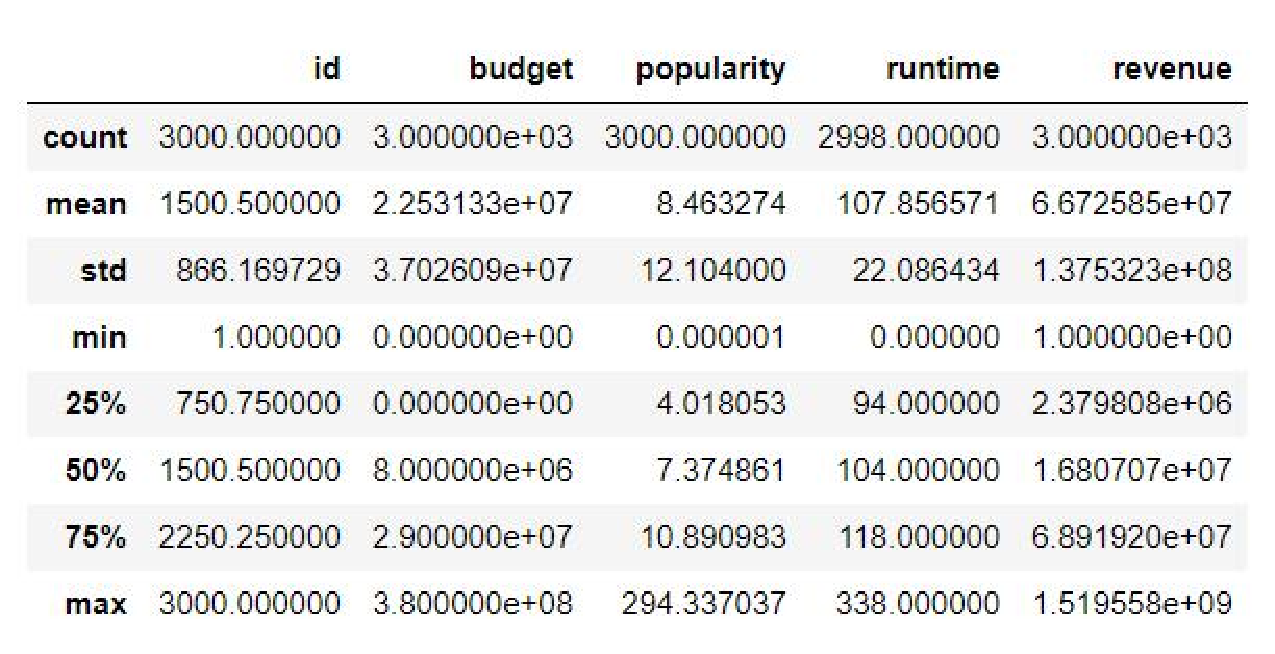
\includegraphics[width=0.7\textwidth,height=0.4\textwidth]{figures/describe.eps}\\
  \caption{Numerical features}
\end{figure}

%%==========================================================================================
\begin{note}
However,
there is such a phenomenon in real life.
Doctors desire to identify the characteristics between
a group of cancer patients and normal people.
NBA coaches are passionate about exploring the obvious strengths and
weaknesses of the team compared with other teams.

Based on such a phenomenon in the real life,
we proposed the concept of group outlying aspects mining.
\end{note}
%%==========================================================================================

\end{slide}
%%==========================================================================================
%%
\begin{slide}{Missing Value}
  \begin{itemize}
    \item
    Remove columns that contain many null-valued features. 
    \item 
    Remove Some columns from which 'Prediction of Revenue' doesn't affect. 
  \end{itemize}
  \vspace{0.75cm}

\twocolumn{
\begin{figure}
  \centering
  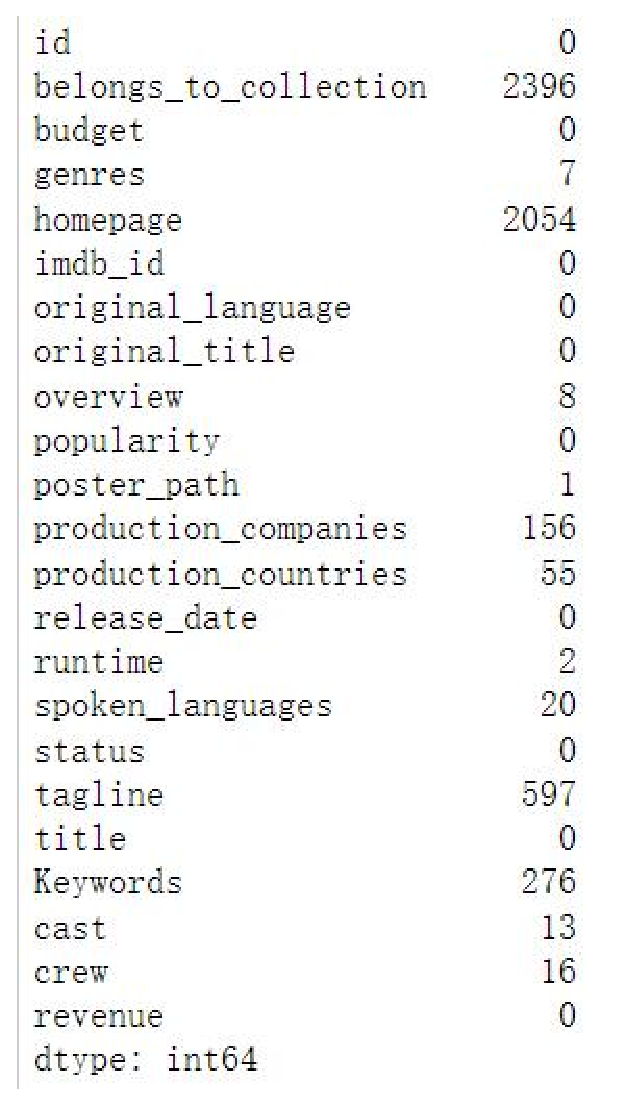
\includegraphics[width=0.5\linewidth]{figures/MissingValue.eps}\\
  \caption{Missing Value}
\end{figure}
}{
\begin{figure}
  \centering
  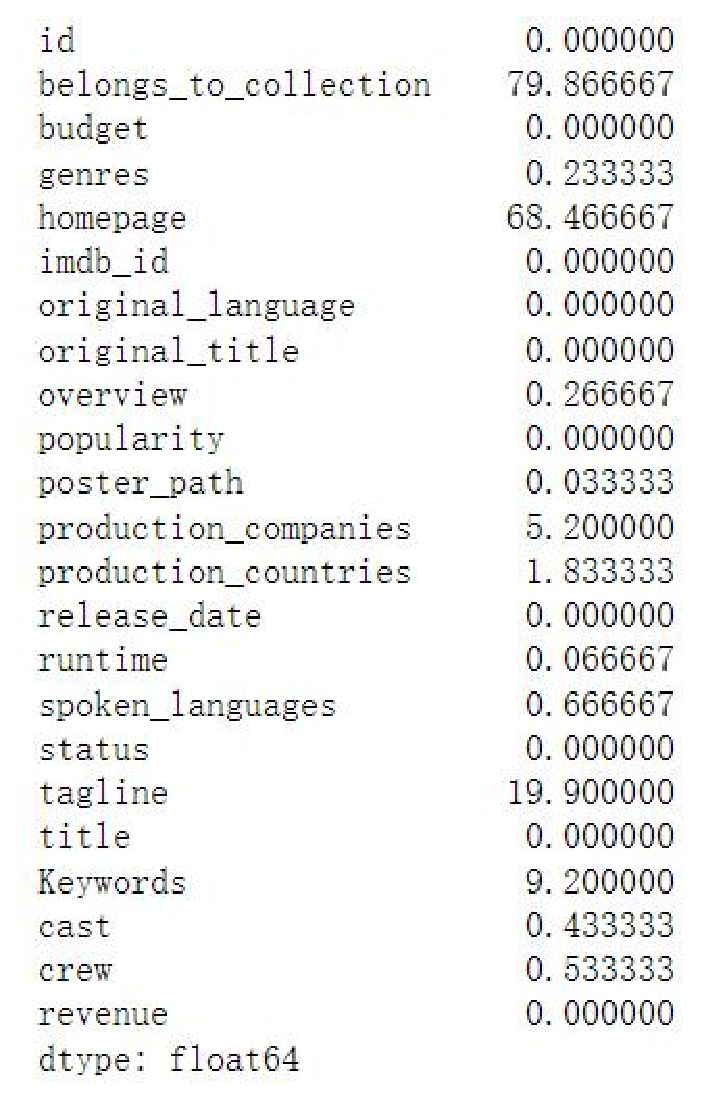
\includegraphics[width=0.58\linewidth]{figures/MissingValuePer.eps}\\
  \caption{Percentage of Missing Value}
\end{figure}
}

%%==========================================================================================
\begin{note}
However,
there is such a phenomenon in real life.
Doctors desire to identify the characteristics between
a group of cancer patients and normal people.
NBA coaches are passionate about exploring the obvious strengths and
weaknesses of the team compared with other teams.

Based on such a phenomenon in the real life,
we proposed the concept of group outlying aspects mining.
\end{note}
%%==========================================================================================

\end{slide}
%%
%%==========================================================================================
%%
\begin{slide}{Genres}
  \begin{itemize}
    \item
    Parse genres in type of JSON format. 
  \end{itemize}
  \begin{figure}[htbp]
    \centering
    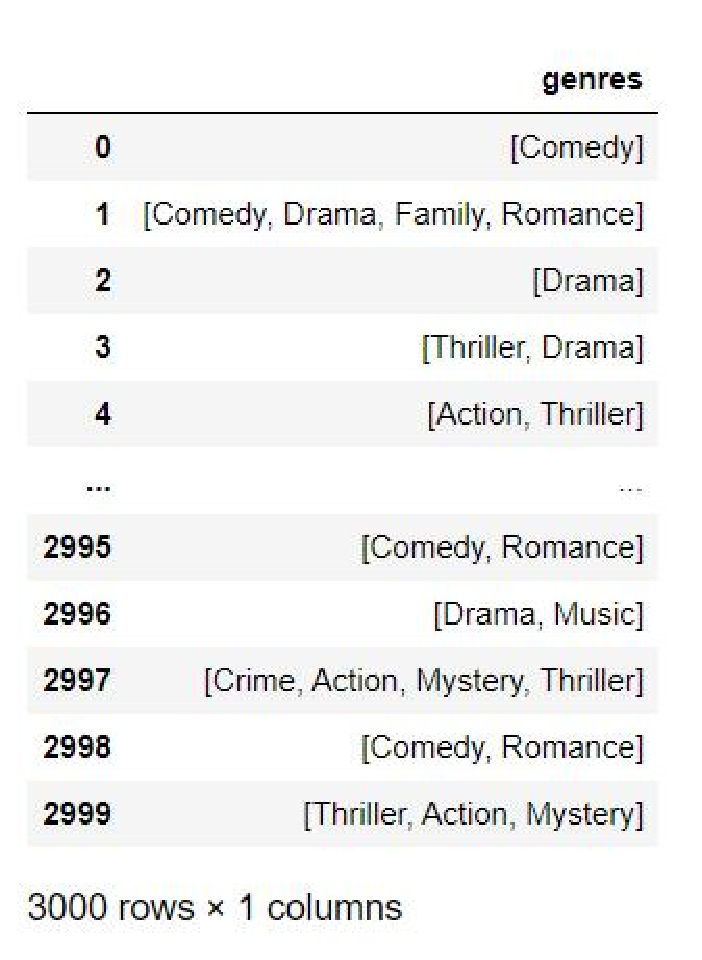
\includegraphics[width=0.5\textwidth,height=0.48\textwidth]{figures/genres.eps}\\
    \caption{genres}
  \end{figure}

%%==========================================================================================
\begin{note}
However,
there is such a phenomenon in real life.
Doctors desire to identify the characteristics between
a group of cancer patients and normal people.
NBA coaches are passionate about exploring the obvious strengths and
weaknesses of the team compared with other teams.

Based on such a phenomenon in the real life,
we proposed the concept of group outlying aspects mining.
\end{note}
%%==========================================================================================

\end{slide}
%%==========================================================================================
%%==========================================================================================
%%
\begin{slide}{Release date}
  \begin{itemize}
    \item
    Parse release date. 
  \end{itemize}
 \vspace{0.5cm}
  \begin{figure}[htbp]
    \centering
    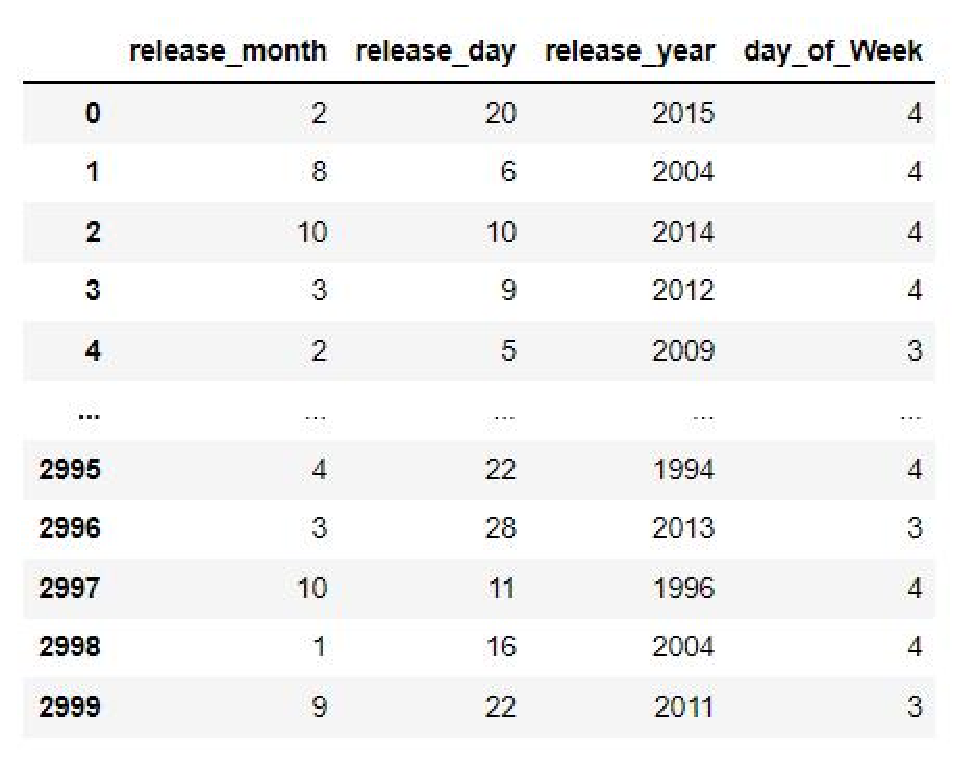
\includegraphics[width=0.6\textwidth,height=0.45\textwidth]{figures/date1.eps}\\
    % \caption{plot}
  \end{figure}

%%==========================================================================================
\begin{note}
However,
there is such a phenomenon in real life.    
Doctors desire to identify the characteristics between
a group of cancer patients and normal people.
NBA coaches are passionate about exploring the obvious strengths and
weaknesses of the team compared with other teams.

Based on such a phenomenon in the real life,
we proposed the concept of group outlying aspects mining.
\end{note}
%%==========================================================================================

\end{slide}
%%==========================================================================================
%%
%%
\section{Data Analysis}
\begin{slide}{Budget Vs Revenue}
  % \begin{itemize}
  %   \item
  %   There are 4 numerical features in total. 
  %   \item 
  %   The minimum of budget is 0. 
  %   \item
  %   There are some missing values in the runtime, and the minimum of runtime is 0.
  % \end{itemize}
 \vspace{2cm}
\twocolumn{
\begin{figure}
  \centering
  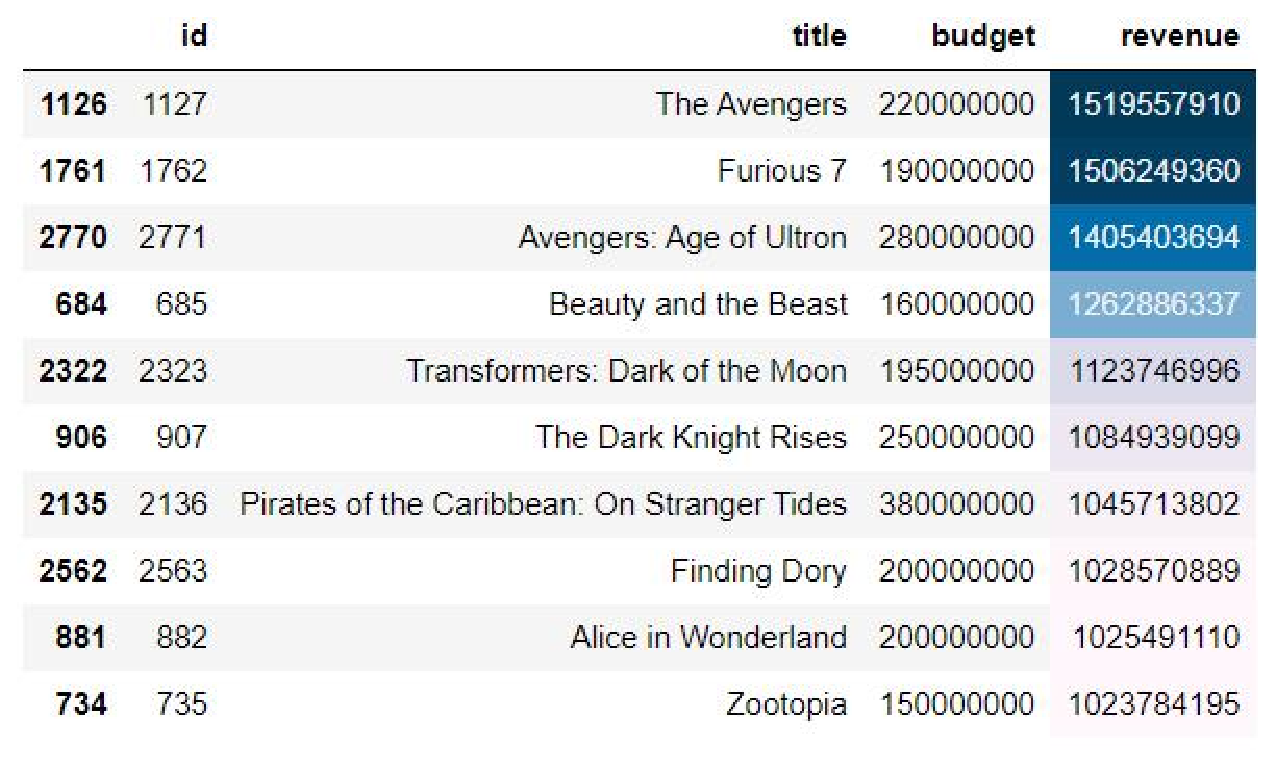
\includegraphics[width=0.9\linewidth,height=0.7\textwidth]{figures/budget1.eps}\\
  \caption{Budget And Revenue}
\end{figure}
}{
\begin{figure}
  \centering
  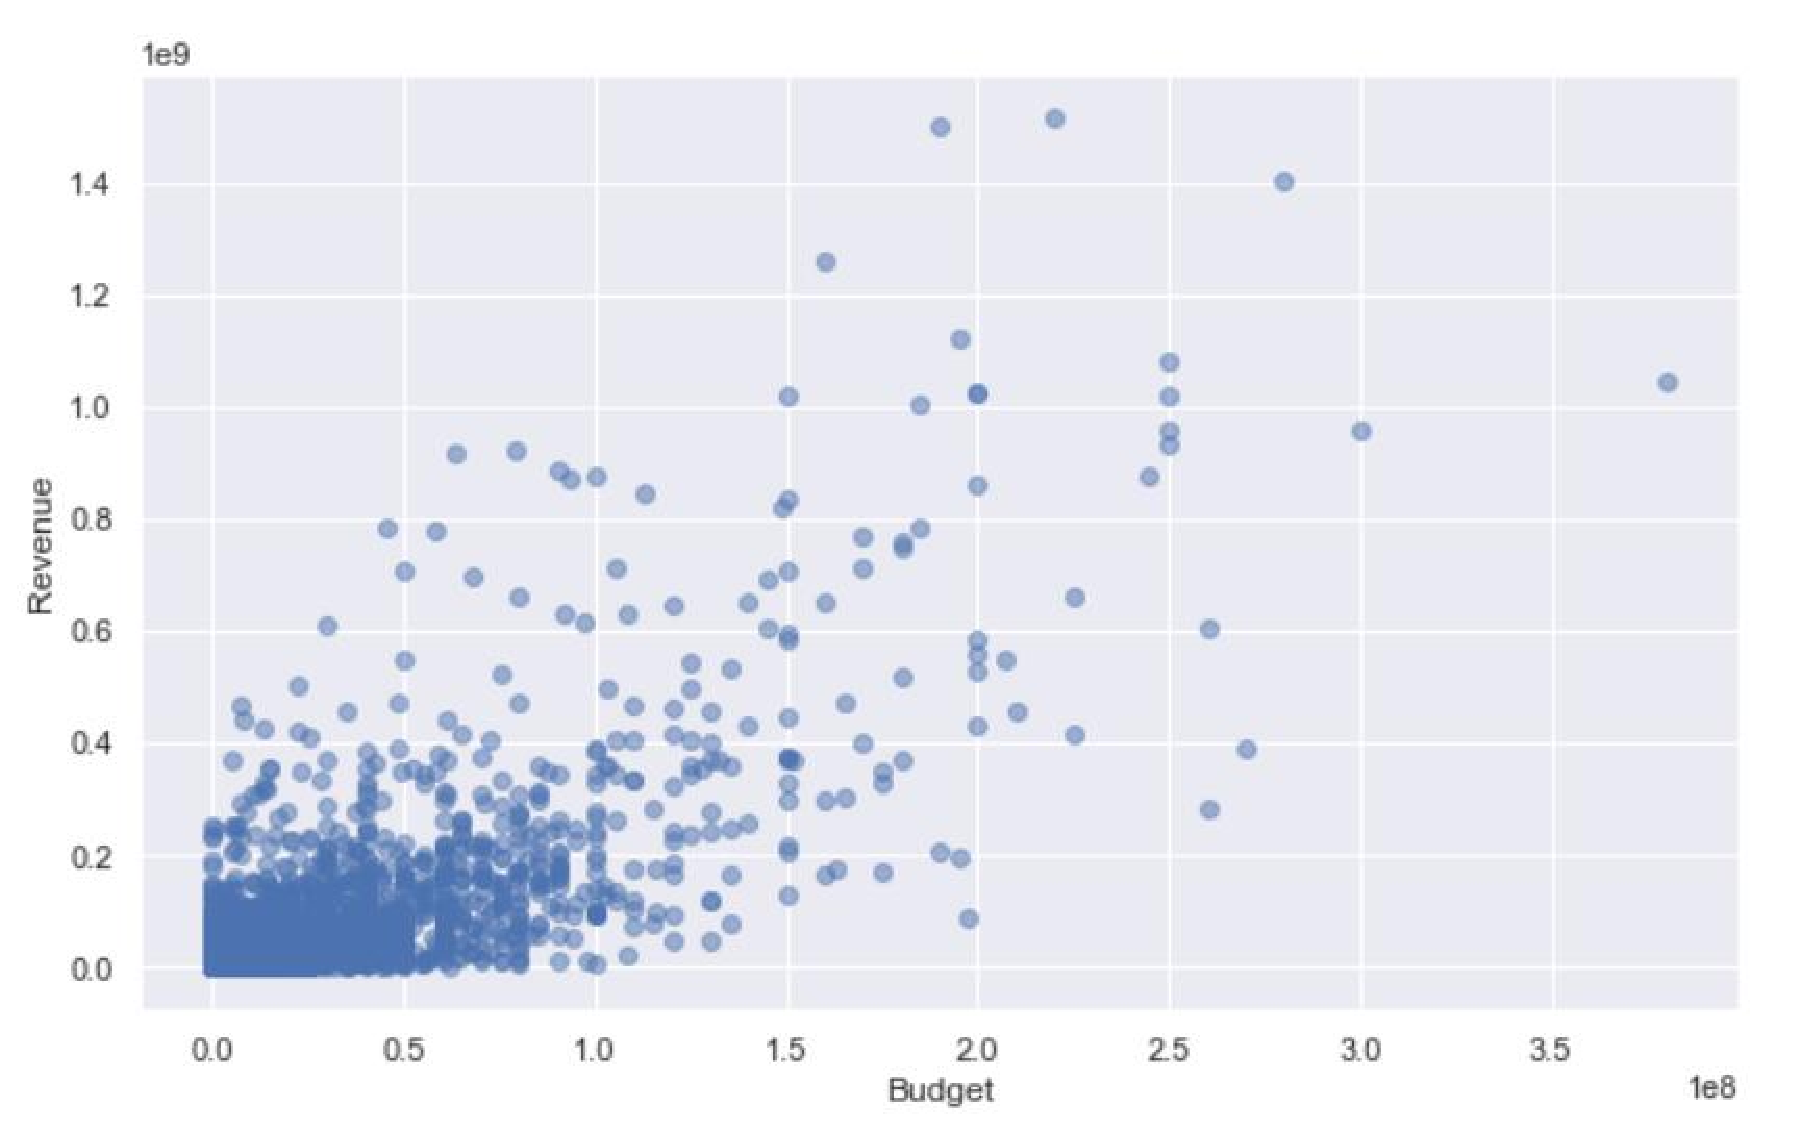
\includegraphics[width=0.9\linewidth,height=0.7\textwidth]{figures/budget2.eps}\\
  \caption{Budget And Revenue Scatter Plot}
\end{figure}
}

%%==========================================================================================
\begin{note}
However,
there is such a phenomenon in real life.
Doctors desire to identify the characteristics between
a group of cancer patients and normal people.
NBA coaches are passionate about exploring the obvious strengths and
weaknesses of the team compared with other teams.

Based on such a phenomenon in the real life,
we proposed the concept of group outlying aspects mining.
\end{note}
%%==========================================================================================

\end{slide}
%%==========================================================================================
%%
\begin{slide}{Popularity Vs Revenue}
  % \begin{itemize}
  %   \item
  %   There are 4 numerical features in total. 
  %   \item 
  %   The minimum of budget is 0. 
  %   \item
  %   There are some missing values in the runtime, and the minimum of runtime is 0.
  % \end{itemize}
 \vspace{2cm}
\twocolumn{
\begin{figure}
  \centering
  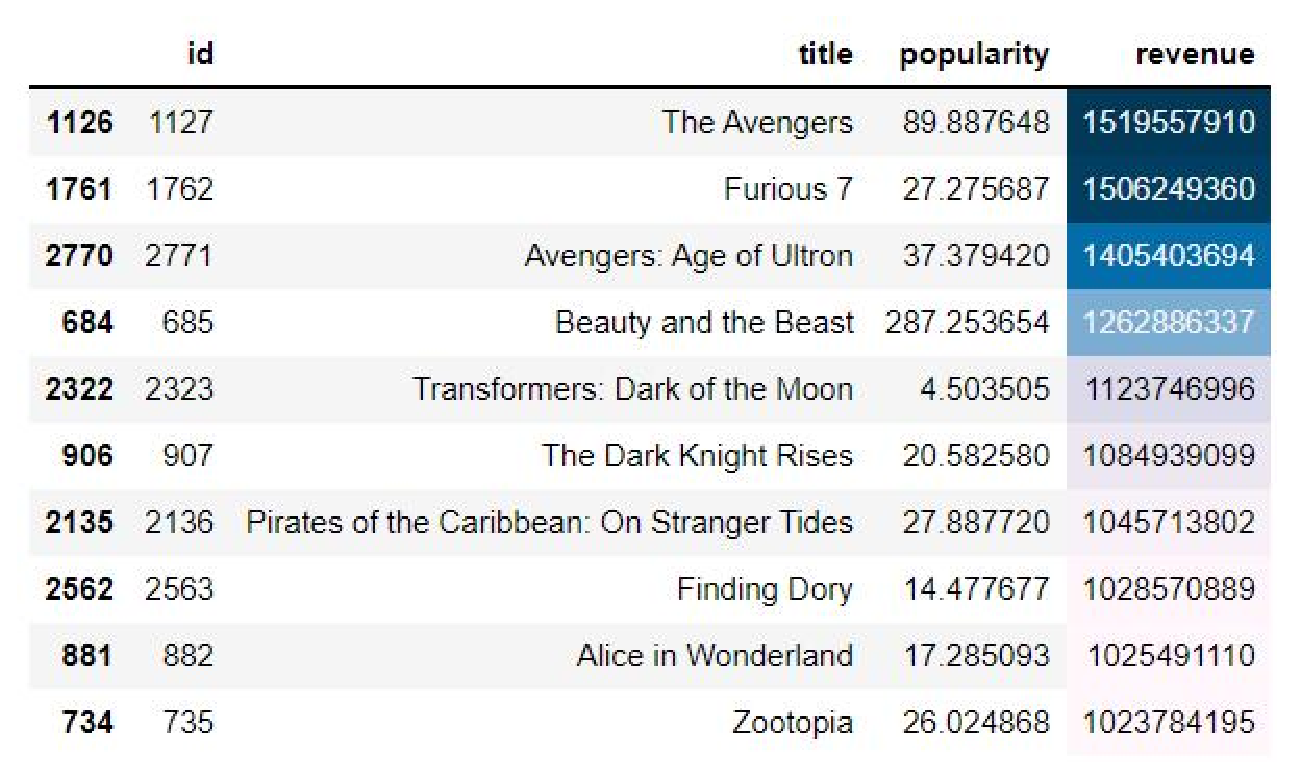
\includegraphics[width=0.9\linewidth,height=0.7\textwidth]{figures/popular1.eps}\\
  \caption{Popularity And Revenue}
\end{figure}
}{
\begin{figure}
  \centering
  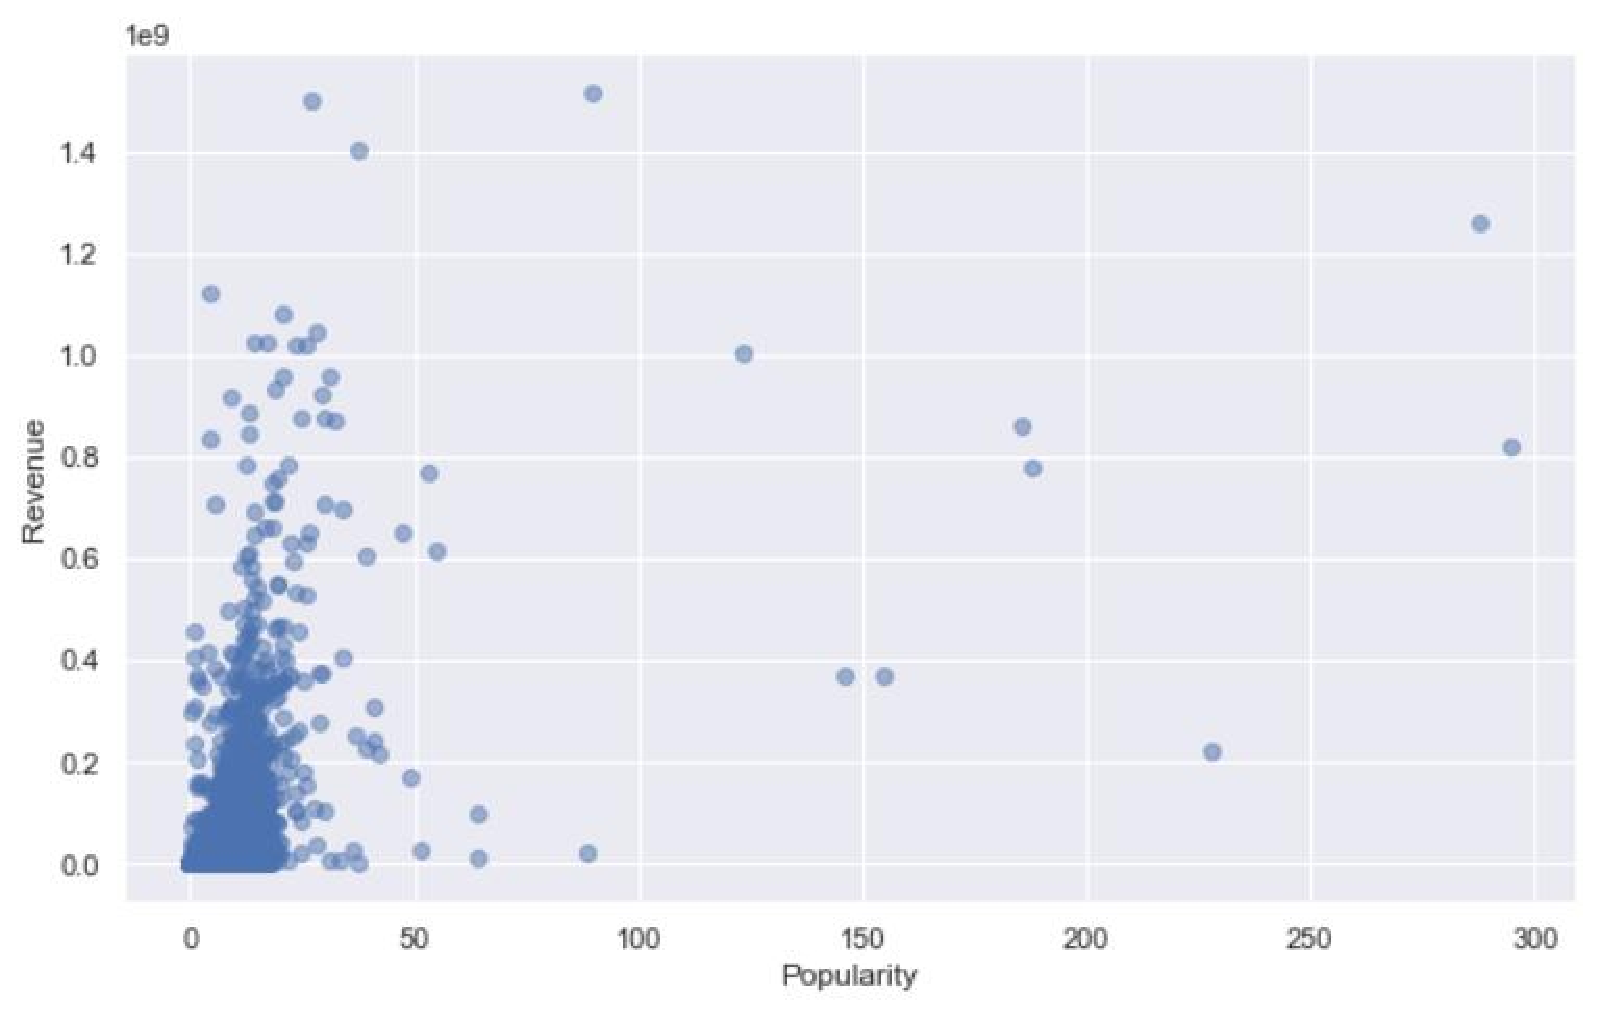
\includegraphics[width=0.9\linewidth,height=0.7\textwidth]{figures/popular2.eps}\\
  \caption{Popularity And Revenue Scatter Plot}
\end{figure}
}

%%==========================================================================================
\begin{note}
However,
there is such a phenomenon in real life.
Doctors desire to identify the characteristics between
a group of cancer patients and normal people.
NBA coaches are passionate about exploring the obvious strengths and
weaknesses of the team compared with other teams.

Based on such a phenomenon in the real life,
we proposed the concept of group outlying aspects mining.
\end{note}
%%==========================================================================================

\end{slide}
%%==========================================================================================
%%==========================================================================================
%%
\begin{slide}{Runtime Vs Revenue}
  \begin{itemize}
    \item
    Most movies are around two hours long. 
    \item 
    View in reverse order of runtime. 
  \end{itemize}
 \vspace{2cm}
\twocolumn{
\begin{figure}
  \centering
  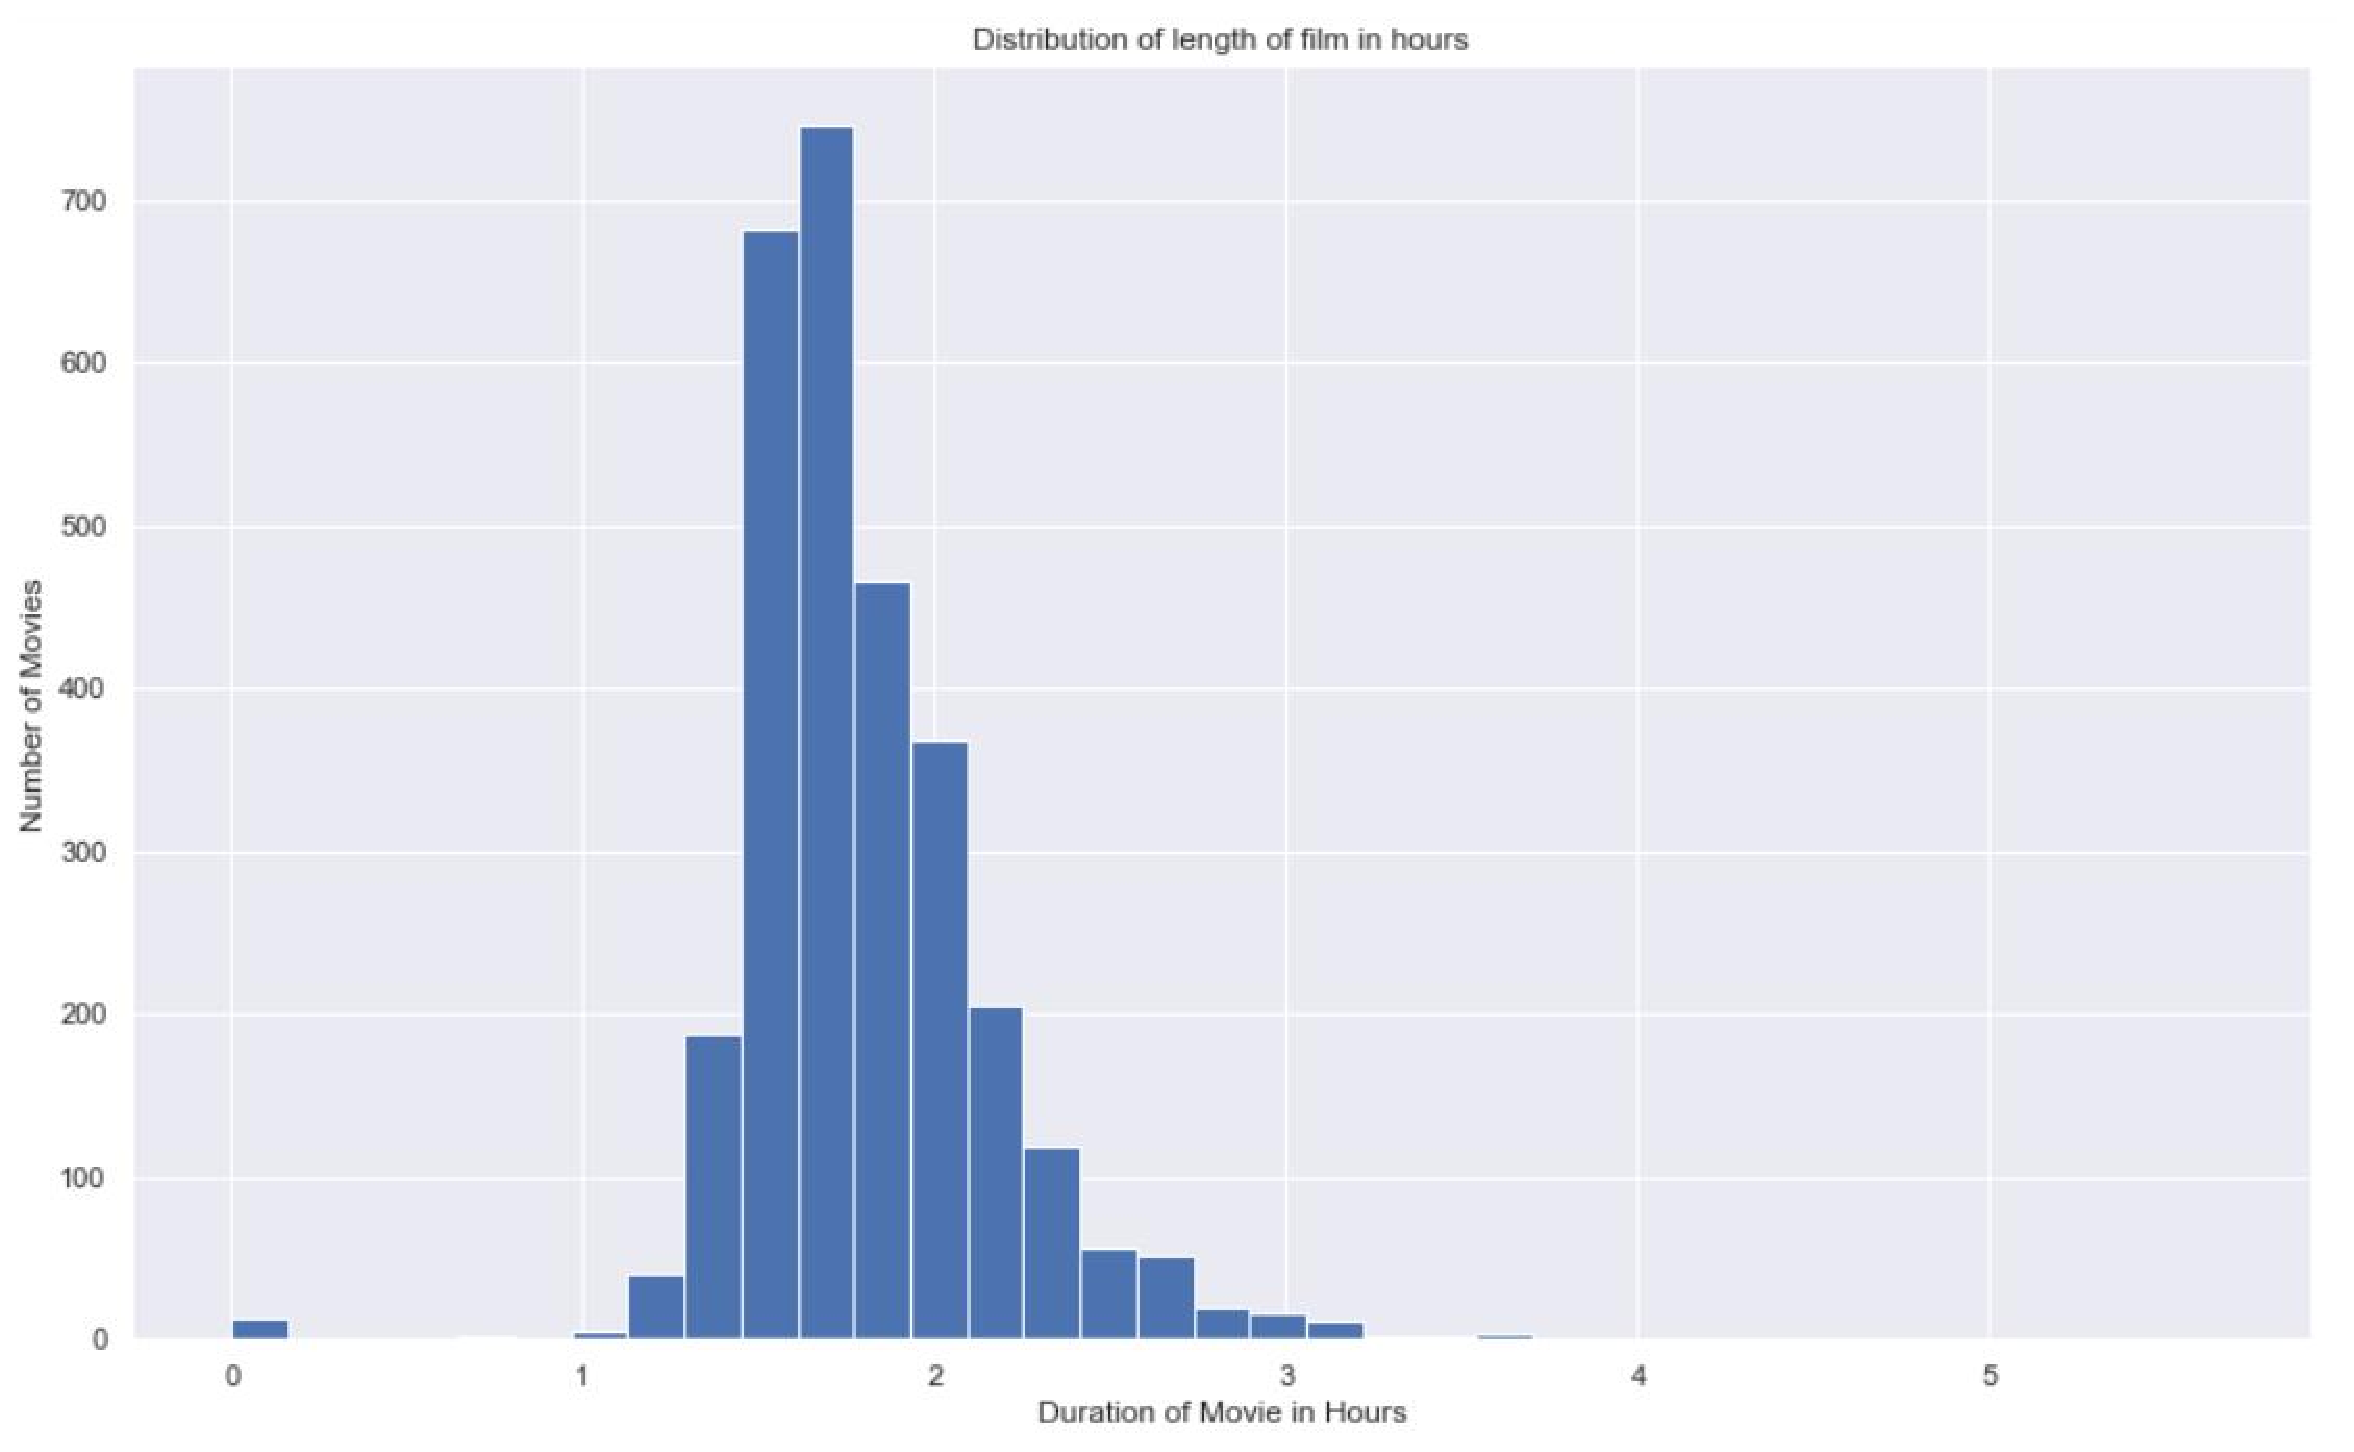
\includegraphics[width=0.9\linewidth,height=0.7\textwidth]{figures/runtime1.eps}\\
  \caption{Runtime  Histogram}
\end{figure}
}{
\begin{figure}
  \centering
  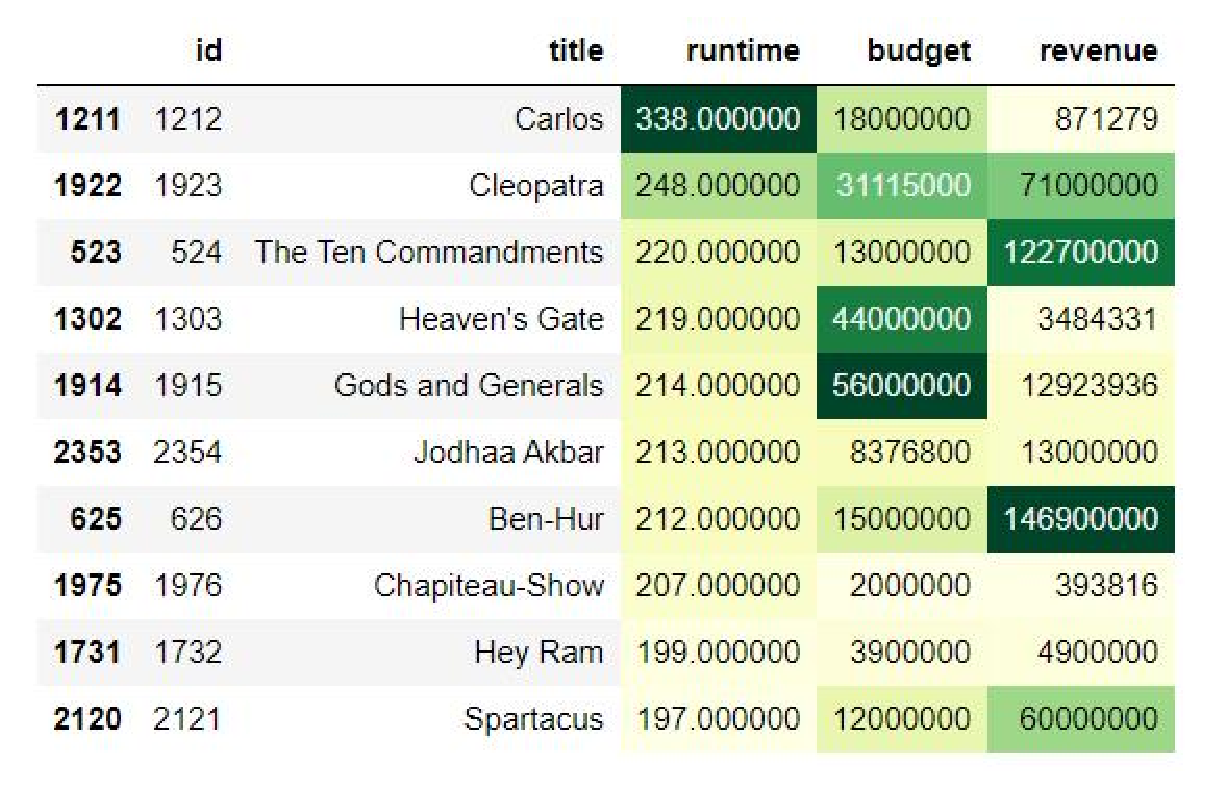
\includegraphics[width=0.9\linewidth,height=0.7\textwidth]{figures/runtime2.eps}\\
  \caption{Runtime And Revenue}
\end{figure}
}

%%==========================================================================================
\begin{note}
However,
there is such a phenomenon in real life.
Doctors desire to identify the characteristics between
a group of cancer patients and normal people.
NBA coaches are passionate about exploring the obvious strengths and
weaknesses of the team compared with other teams.

Based on such a phenomenon in the real life,
we proposed the concept of group outlying aspects mining.
\end{note}
%%==========================================================================================

\end{slide}
%%==========================================================================================
%%

%%==========================================================================================
%%
\begin{slide}{genres}
  \begin{itemize}
    \item
    Drama and comedy dominate. 
  \end{itemize}
 \vspace{0.5cm}
  \begin{figure}[htbp]
    \centering
    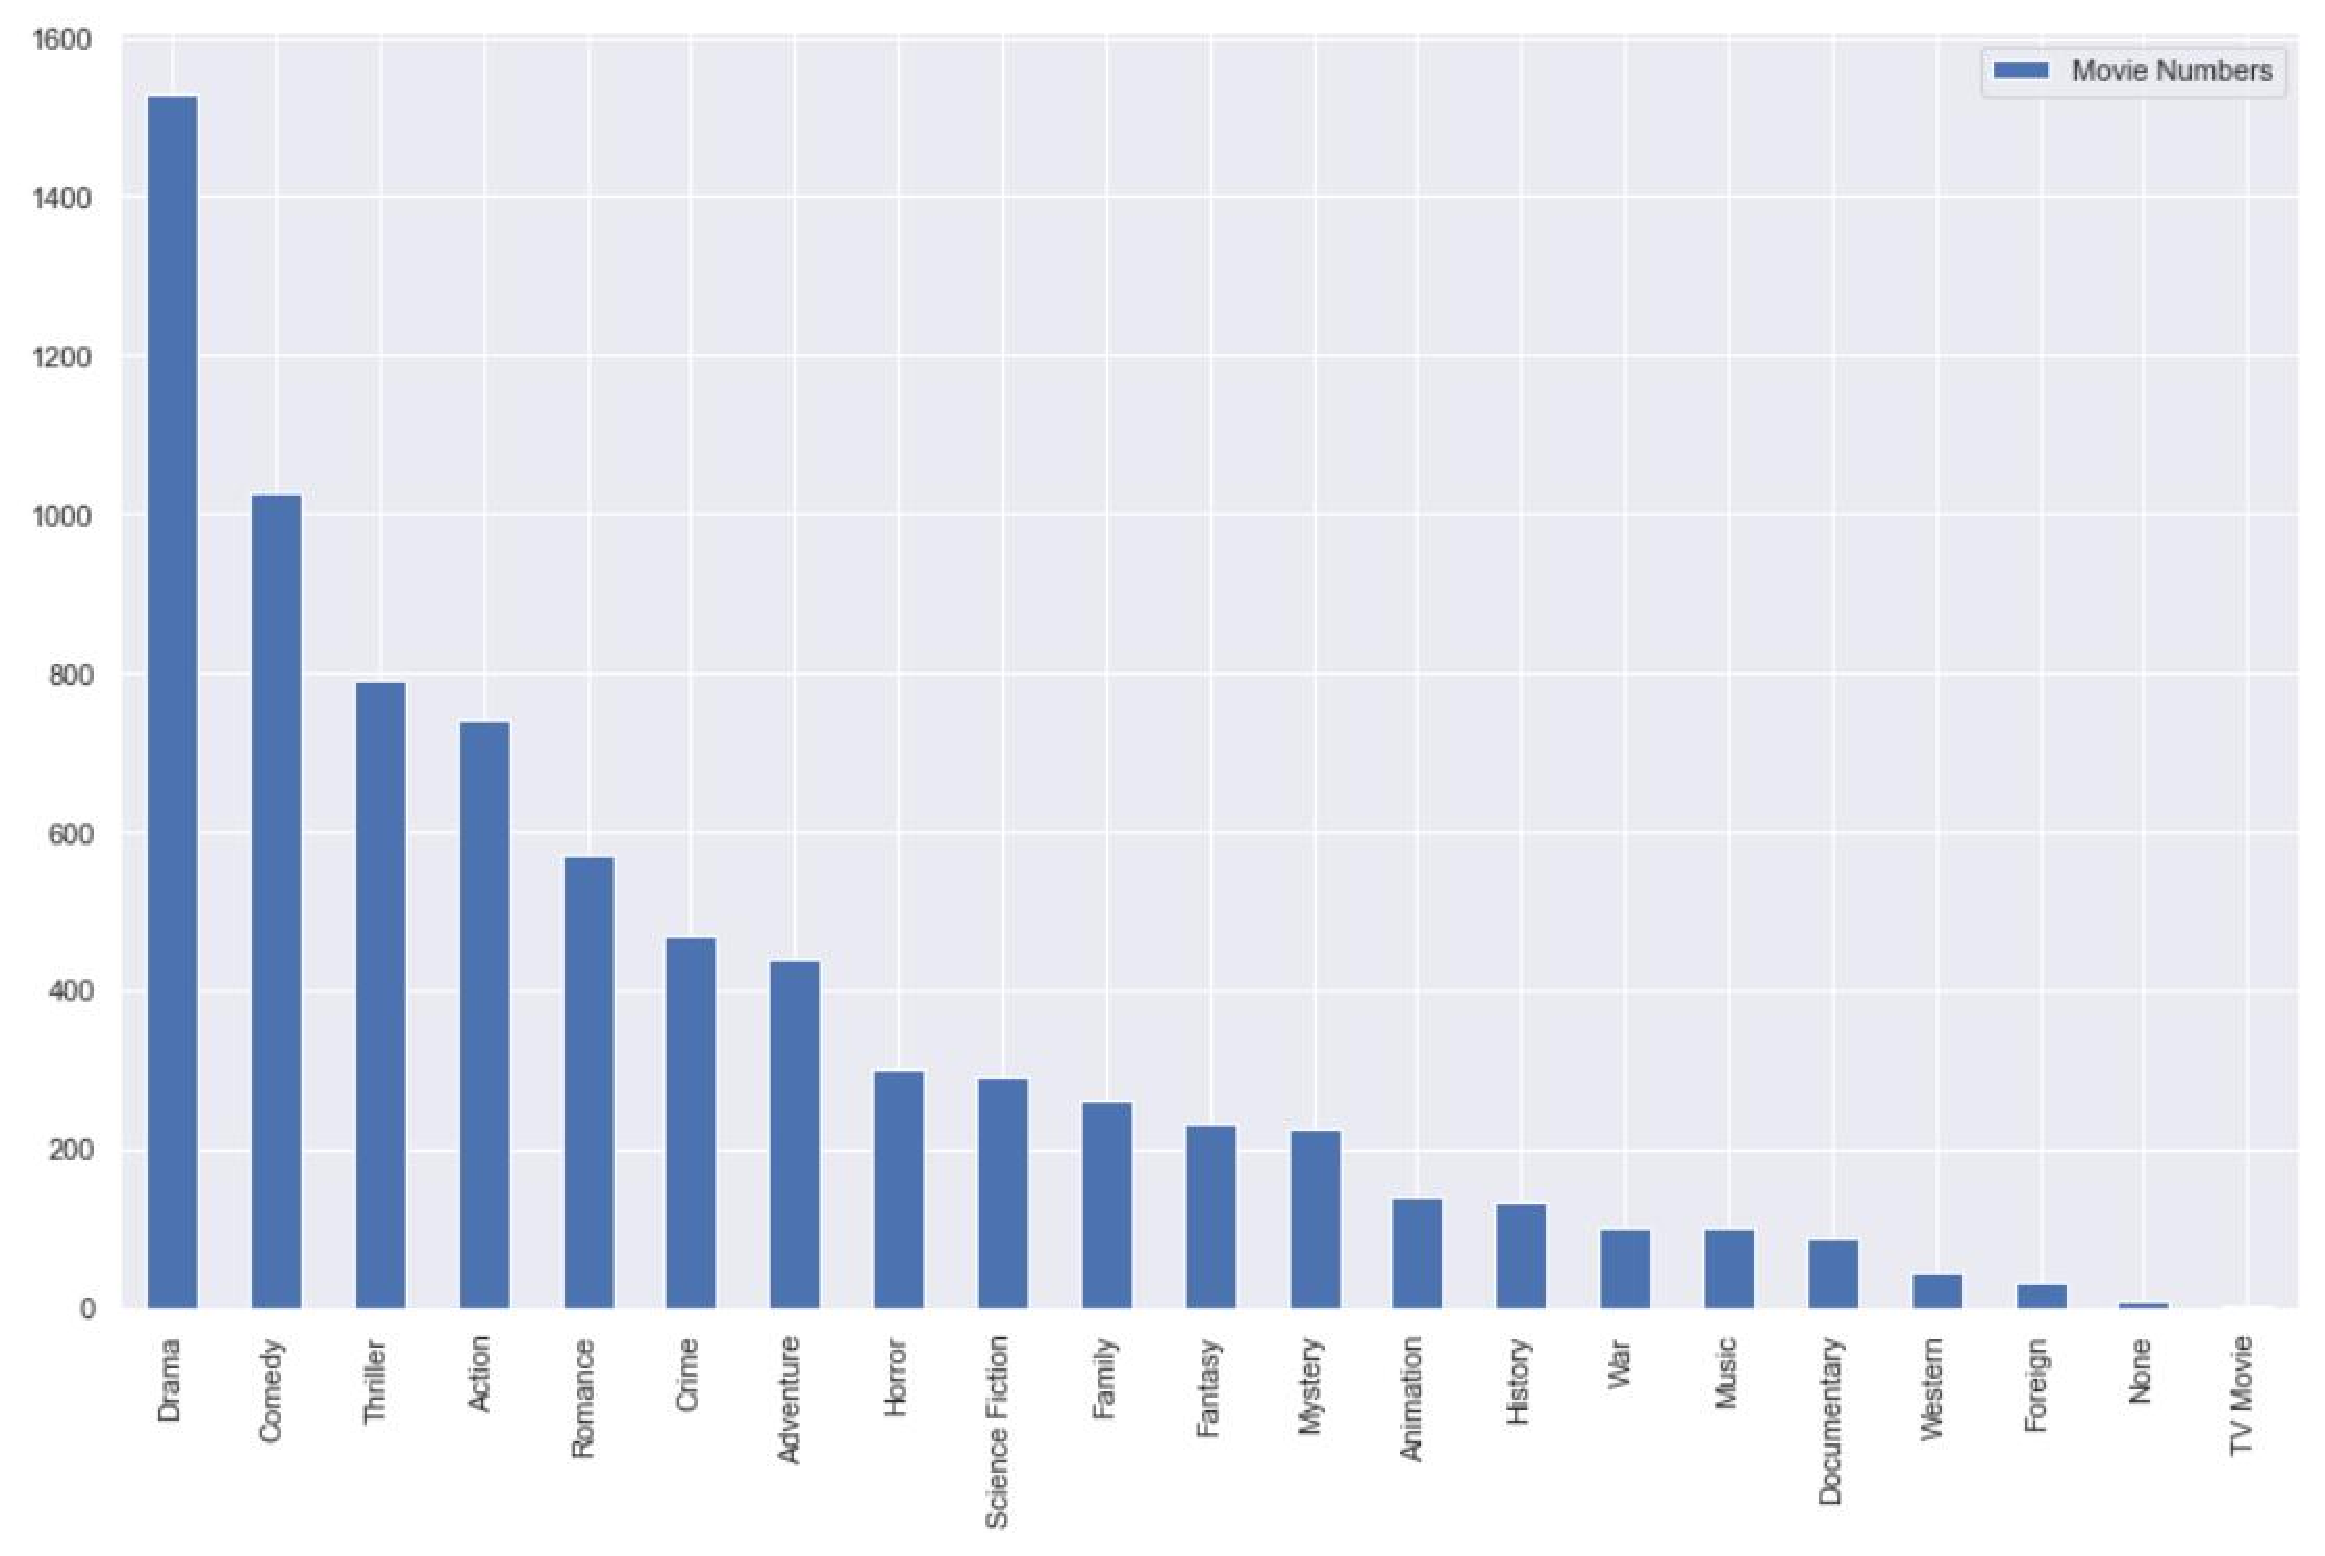
\includegraphics[width=0.6\textwidth,height=0.45\textwidth]{figures/genres1.eps}\\
    \caption{genres bar plot}
  \end{figure}

%%==========================================================================================
\begin{note}
However,
there is such a phenomenon in real life.
Doctors desire to identify the characteristics between
a group of cancer patients and normal people.
NBA coaches are passionate about exploring the obvious strengths and
weaknesses of the team compared with other teams.

Based on such a phenomenon in the real life,
we proposed the concept of group outlying aspects mining.
\end{note}
%%==========================================================================================

\end{slide}

%%==========================================================================================
%%
\begin{slide}{Year And Revenue}
  \begin{itemize}
    \item
    More and more movies have been released in recent years. 
    \item
    There may be a positive correlation between Year and Revenue. 
  \end{itemize}
  \vspace{2cm}
  \twocolumn{
  \begin{figure}
    \centering
    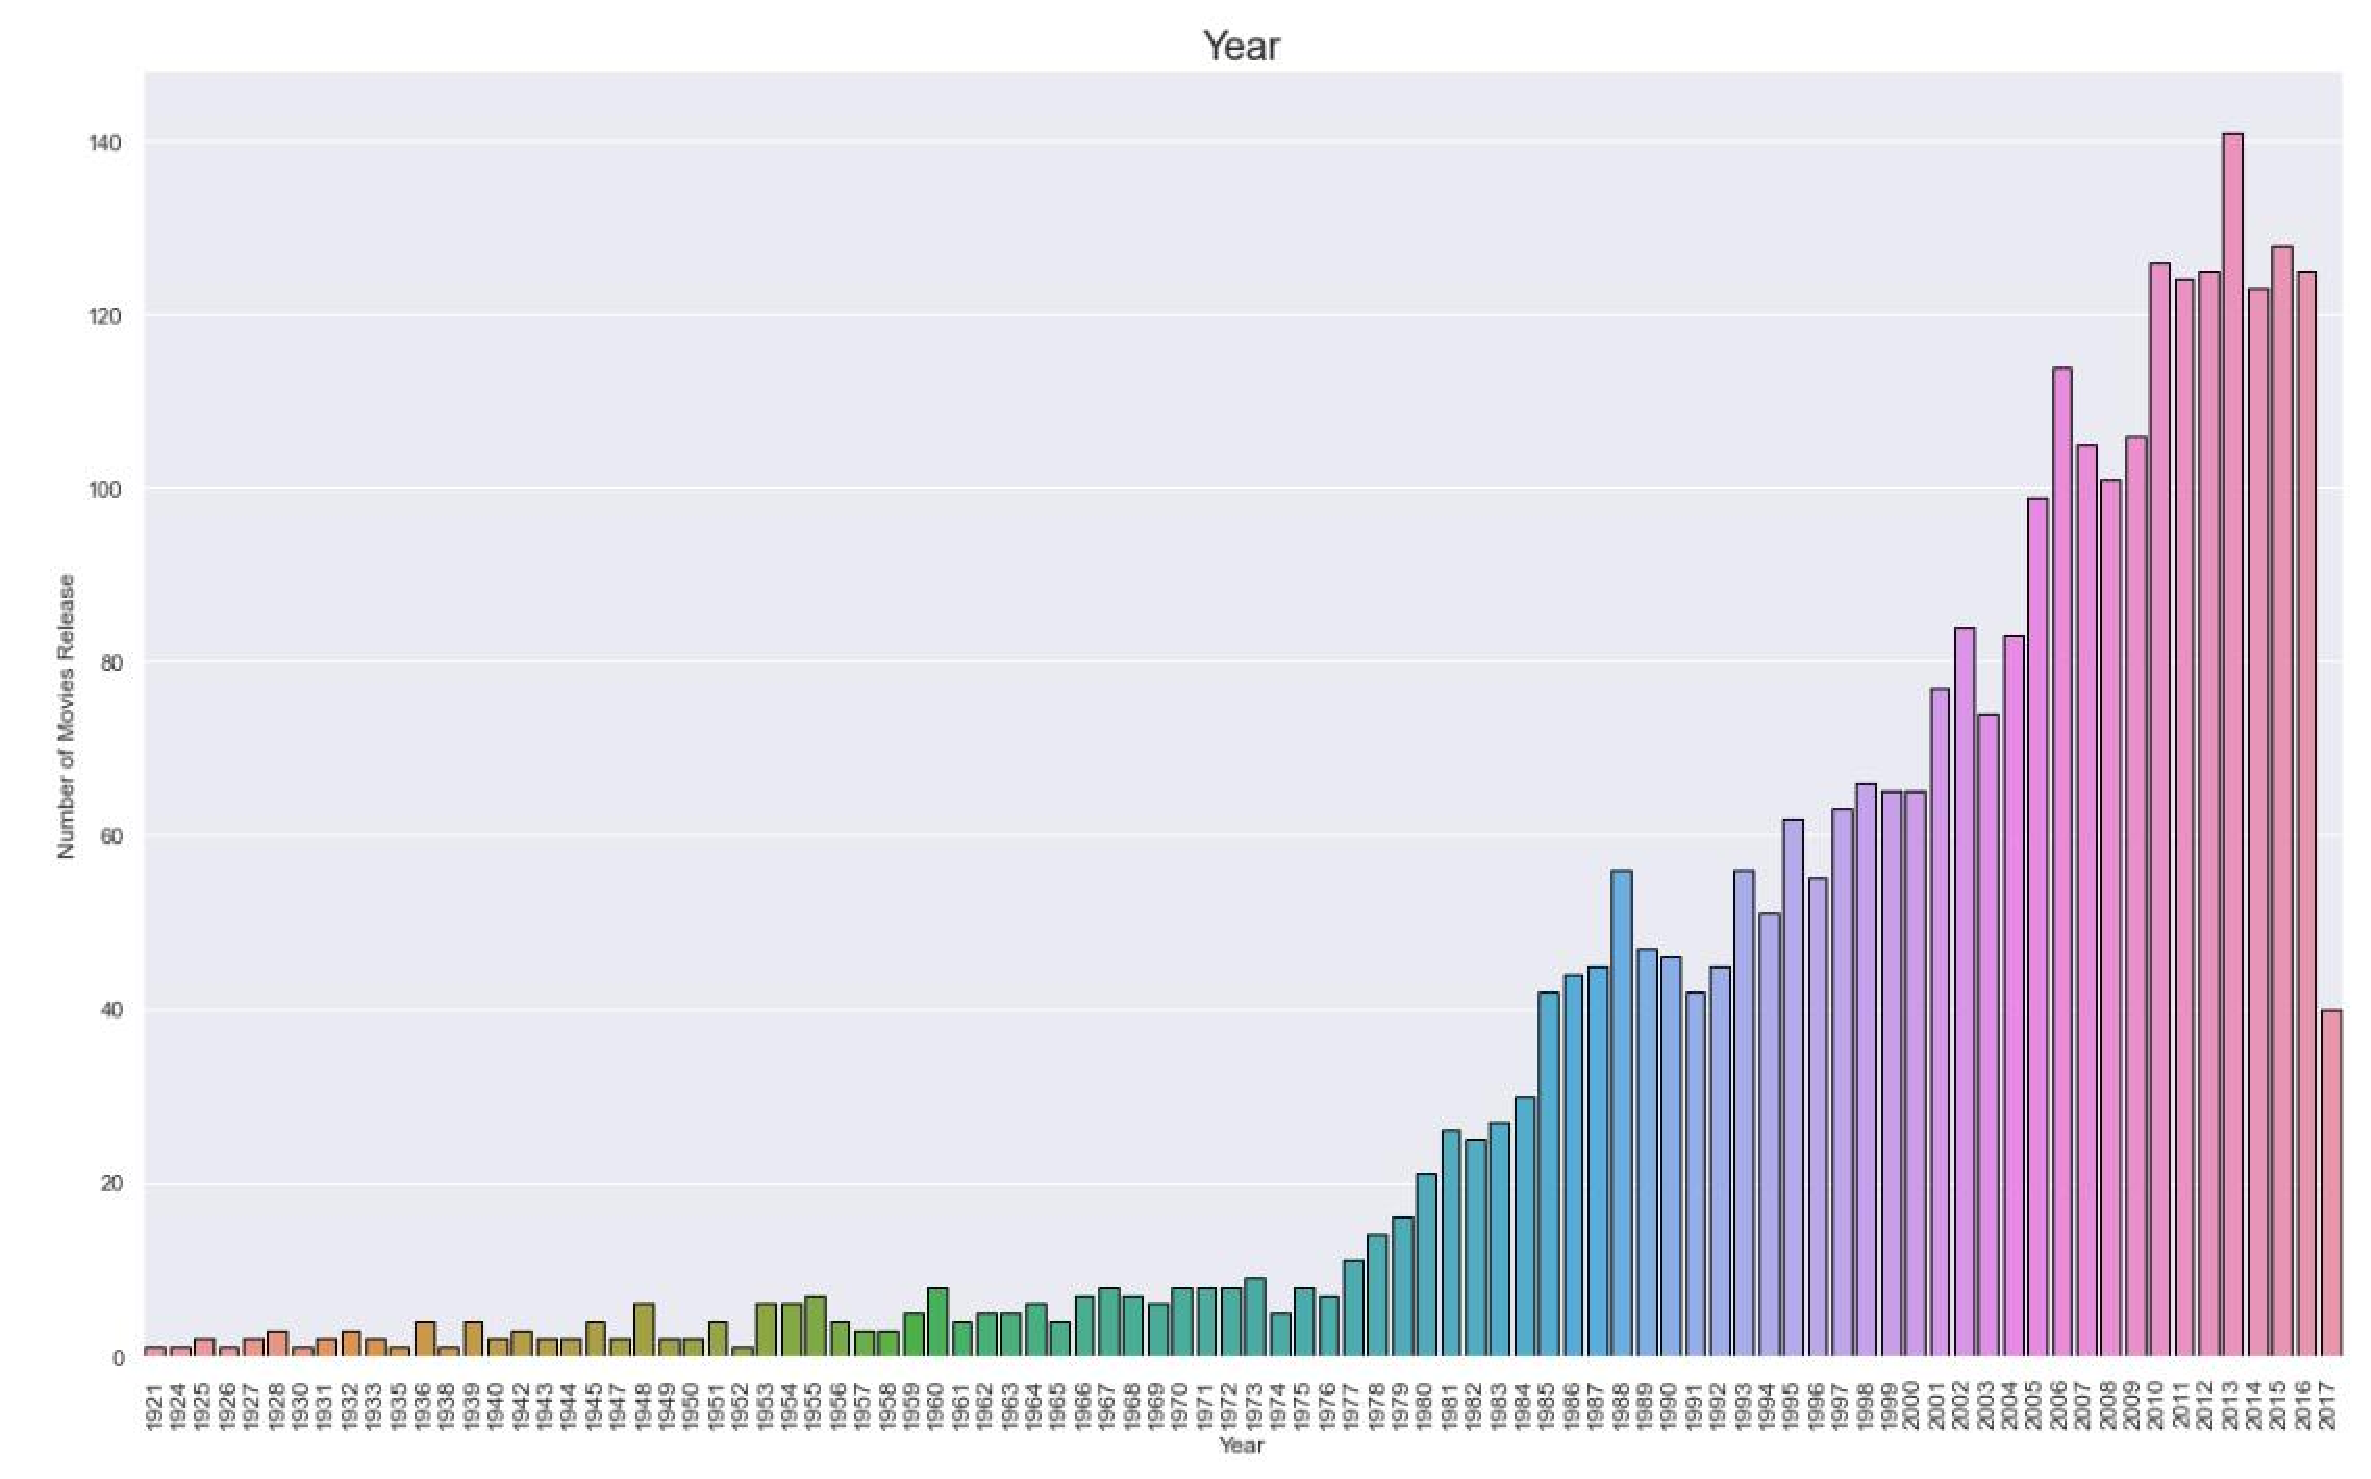
\includegraphics[width=0.95\linewidth,height=0.8\textwidth]{figures/year1.eps}\\
    \caption{Histogram}
  \end{figure}
  }{
  \begin{figure}
    \centering
    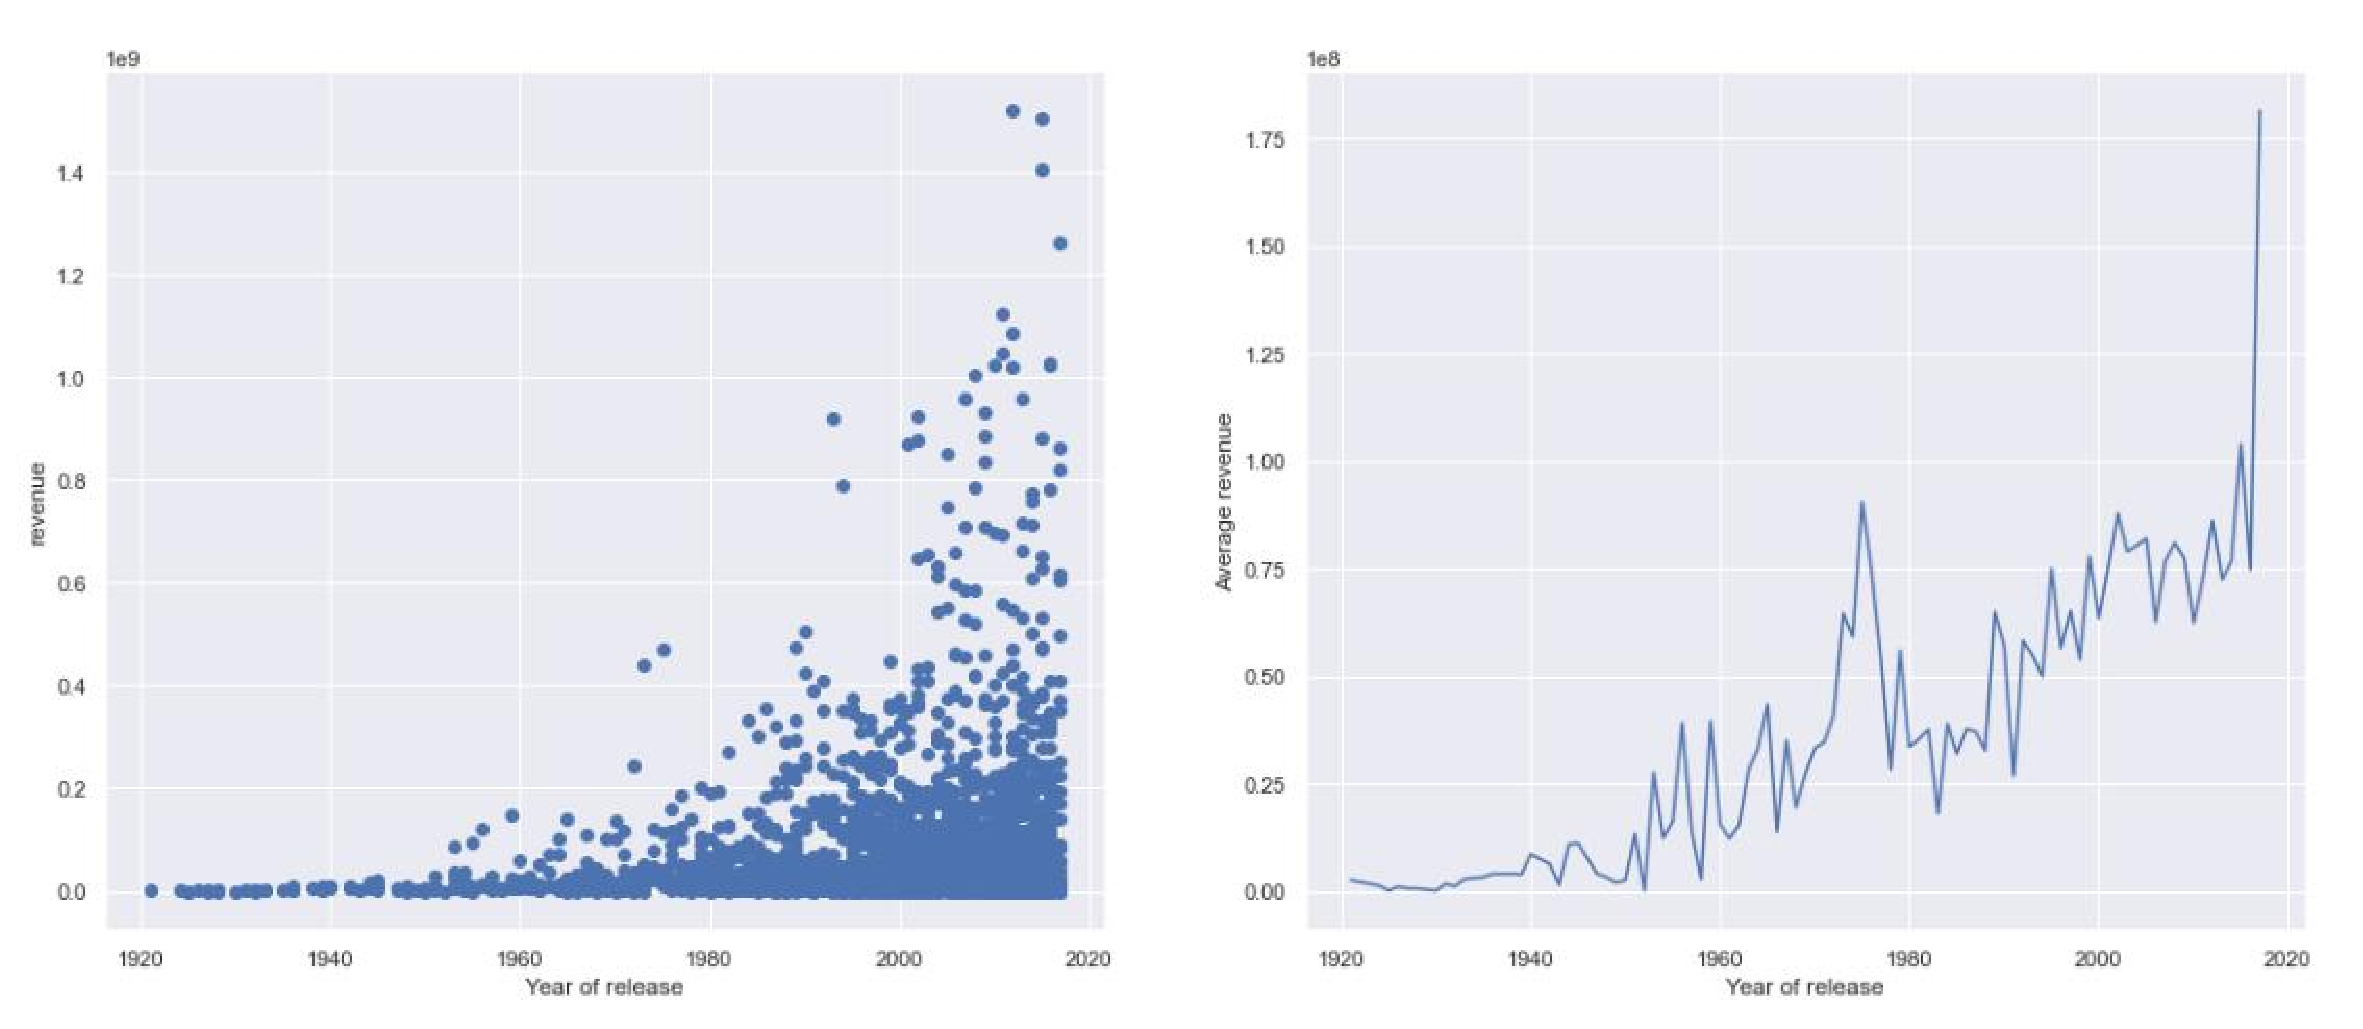
\includegraphics[width=1.0\linewidth,height=0.8\textwidth]{figures/year2.eps}\\
    \caption{Scatter Plot}
  \end{figure}
  }
%%==========================================================================================
\begin{note}
However,
there is such a phenomenon in real life.
Doctors desire to identify the characteristics between
a group of cancer patients and normal people.
NBA coaches are passionate about exploring the obvious strengths and
weaknesses of the team compared with other teams.

Based on such a phenomenon in the real life,
we proposed the concept of group outlying aspects mining.
\end{note}
%%==========================================================================================
\end{slide}

%%==========================================================================================
%%
%%==========================================================================================
%%
\begin{slide}{Month And Week}
  \begin{itemize}
    \item
    The number of movies released in September and October is higher. 
    \item
    The number of films released on Friday accounted for the majority. 
  \end{itemize}
  \vspace{2cm}
  \twocolumn{
  \begin{figure}
    \centering
    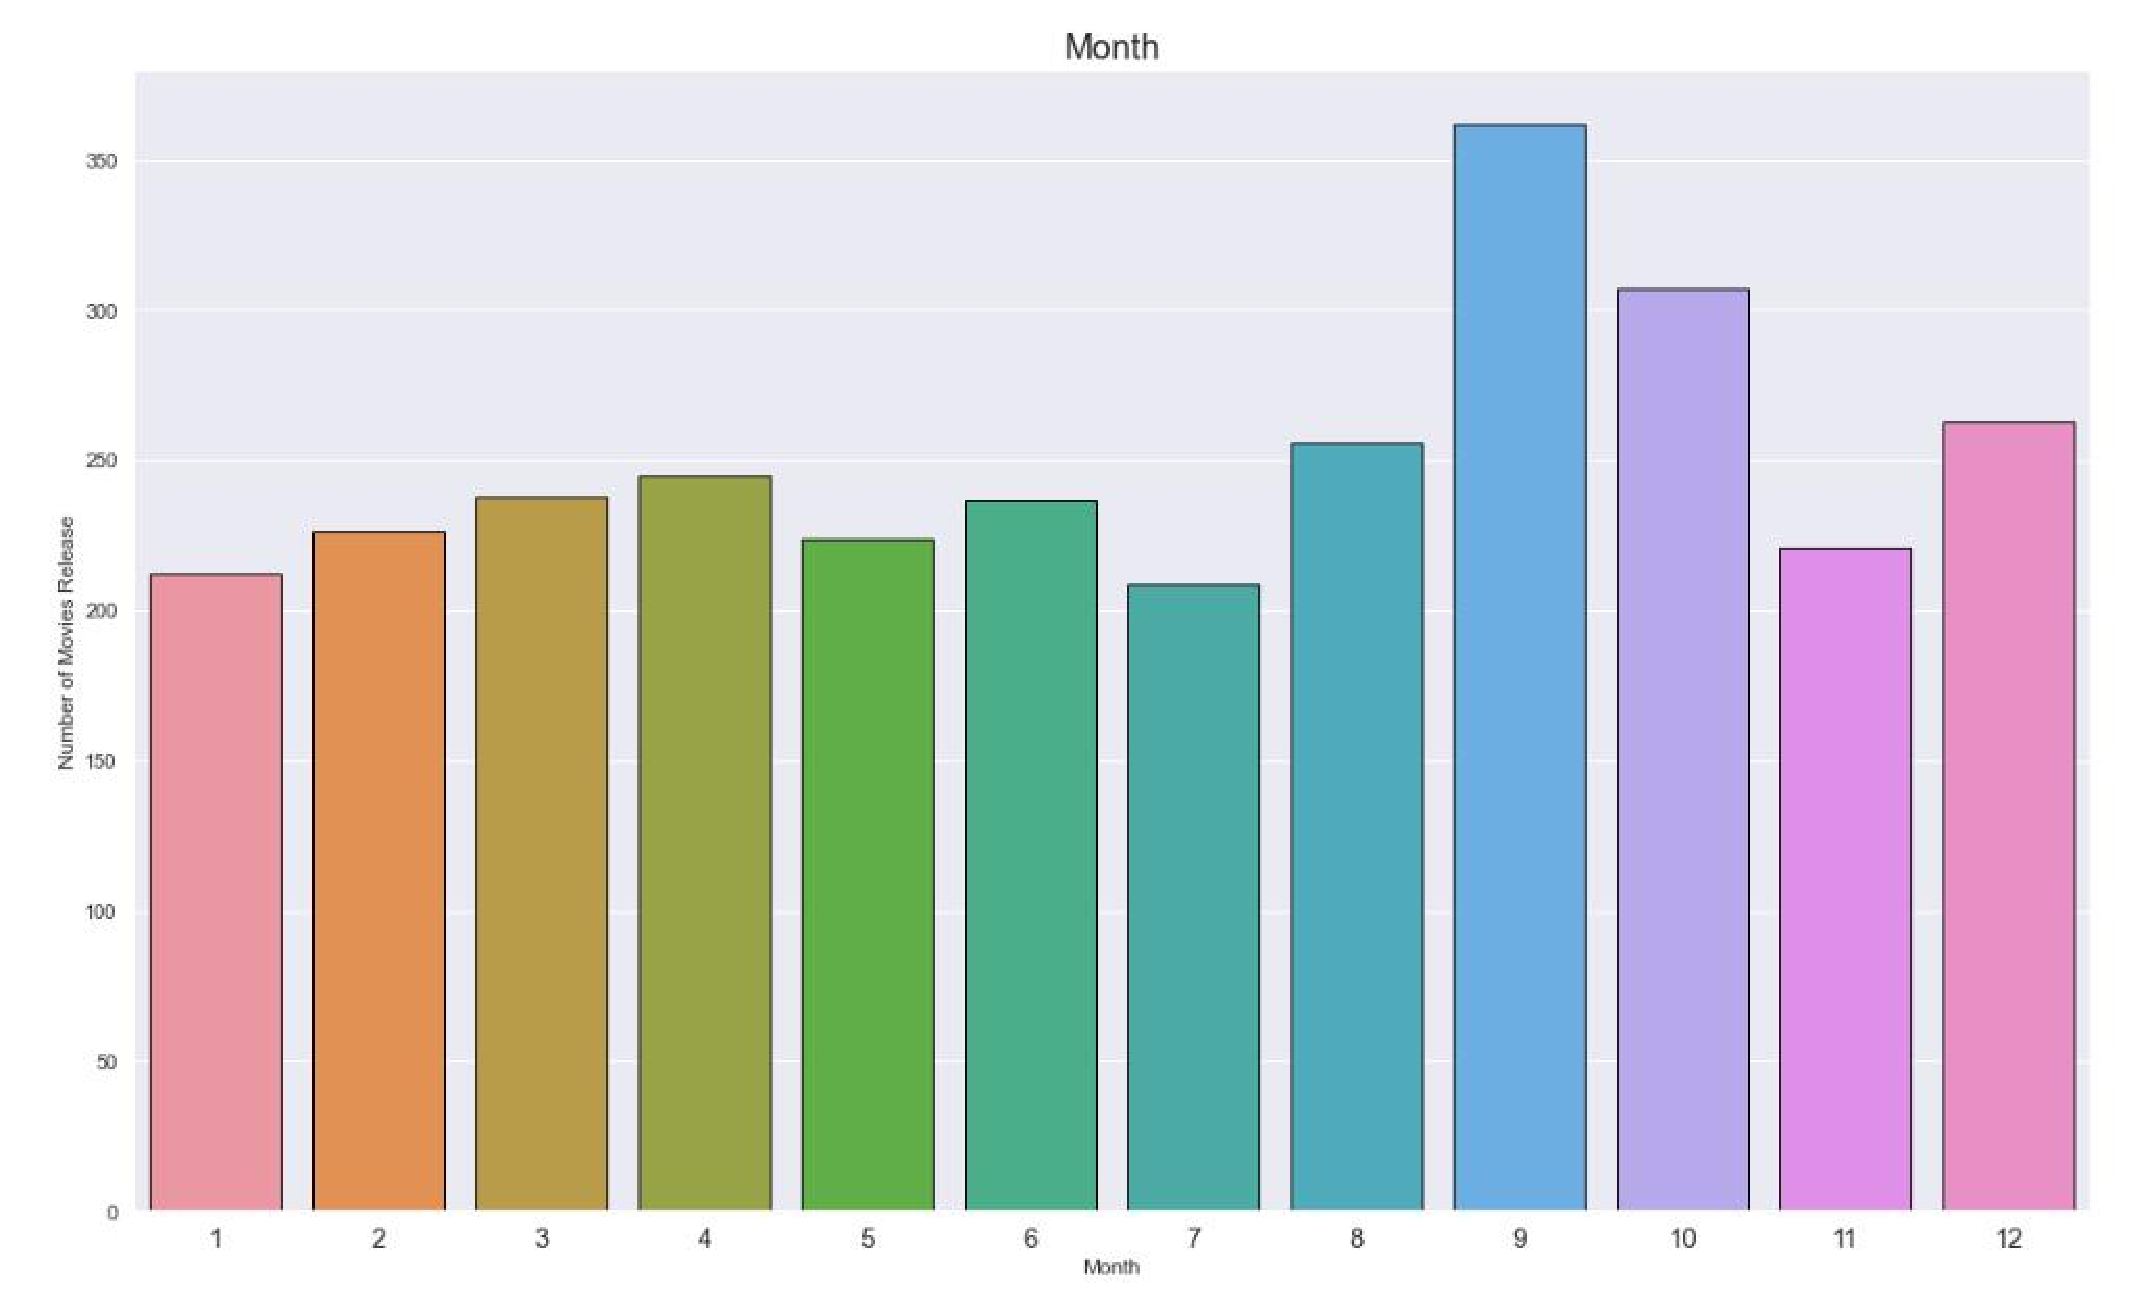
\includegraphics[width=0.95\linewidth,height=0.8\textwidth]{figures/month.eps}\\
    \caption{Month}
  \end{figure}
  }{
  \begin{figure}
    \centering
    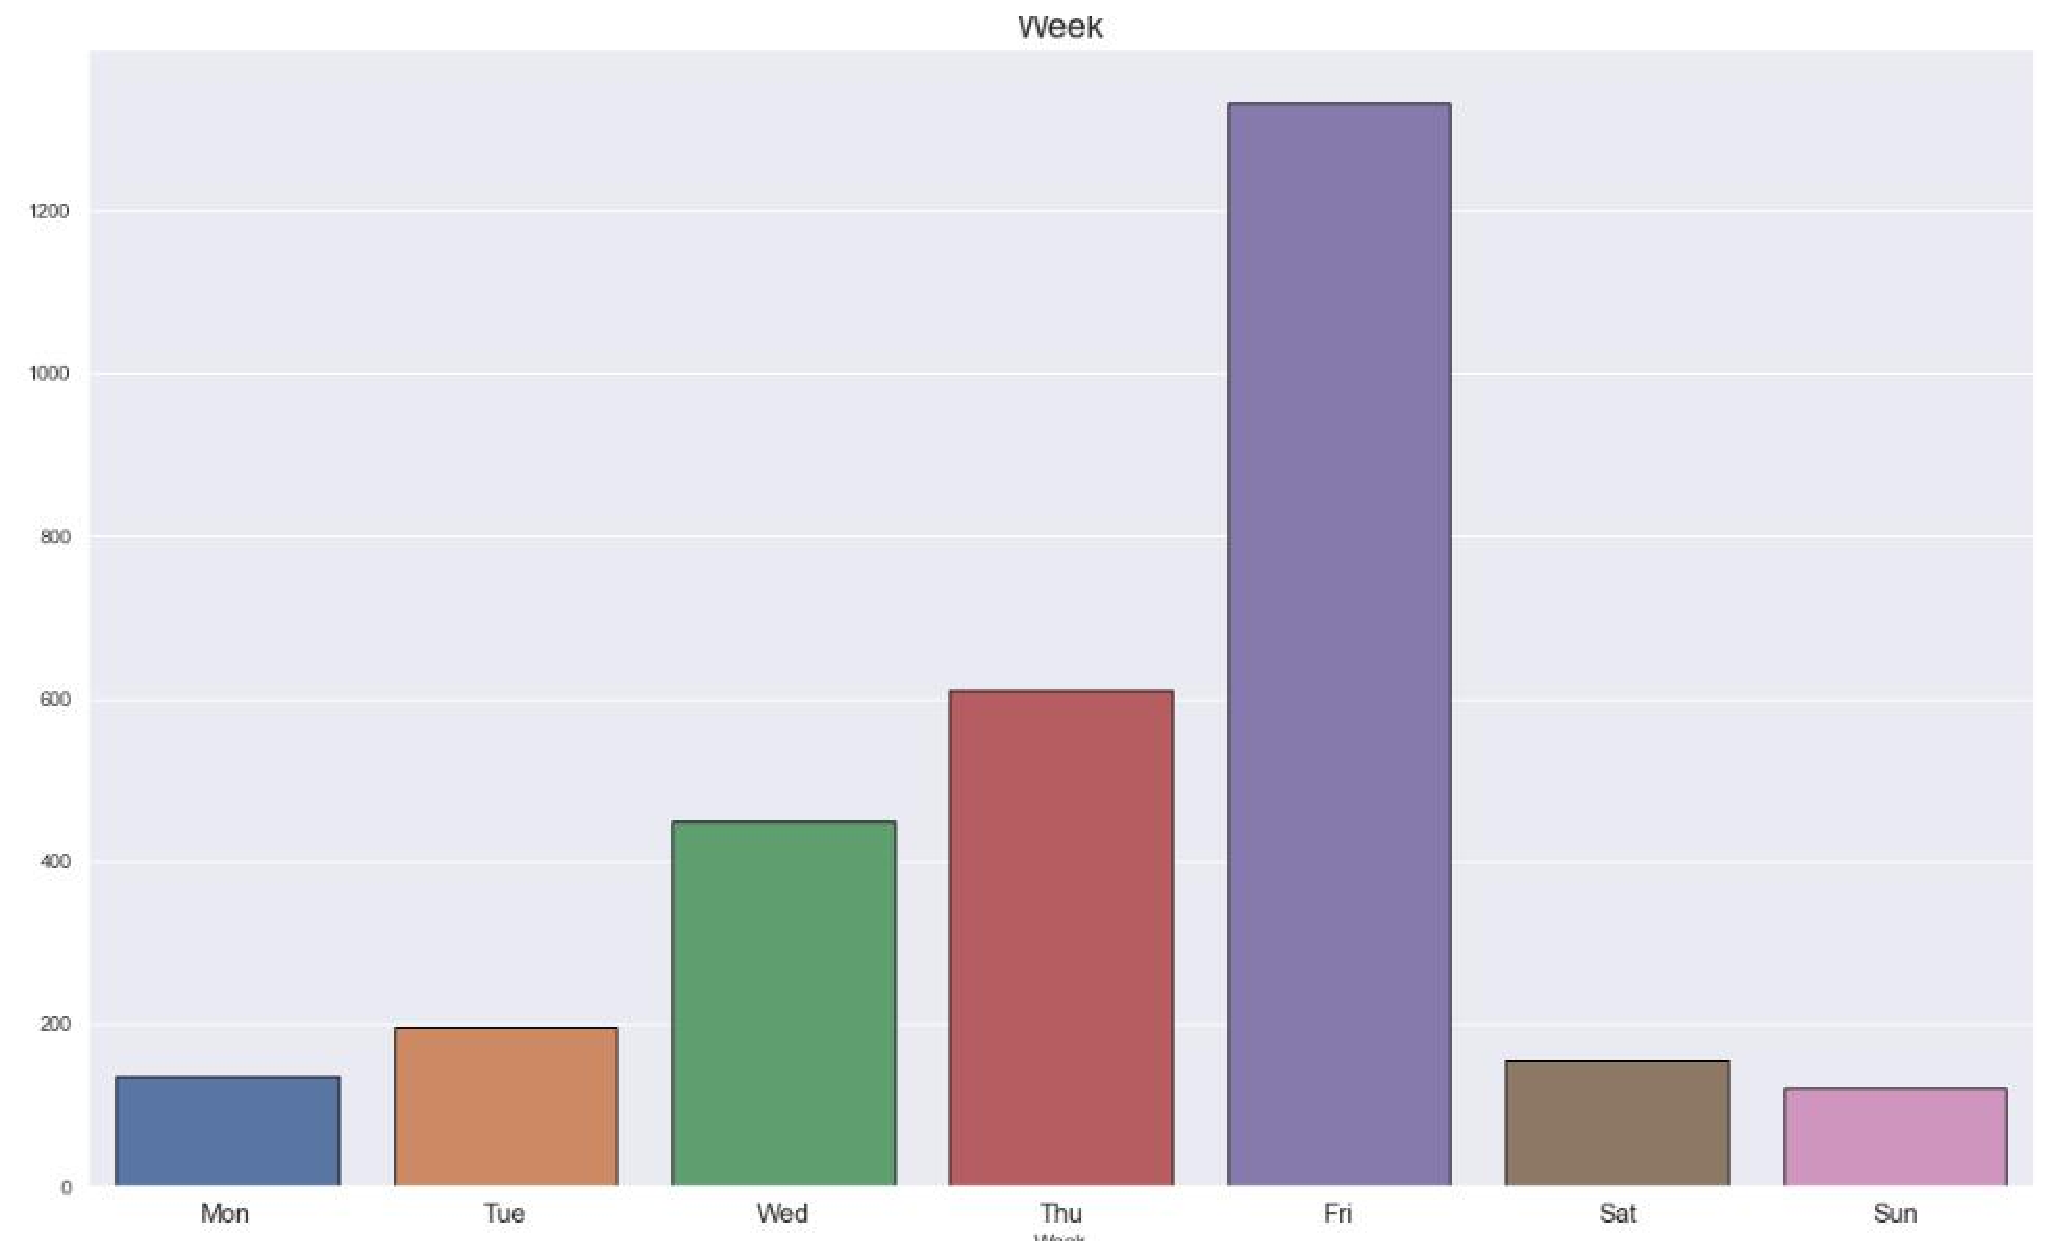
\includegraphics[width=0.95\linewidth,height=0.8\textwidth]{figures/week.eps}\\
    \caption{Week}
  \end{figure}
  }
%%==========================================================================================
\begin{note}
However,
there is such a phenomenon in real life.
Doctors desire to identify the characteristics between
a group of cancer patients and normal people.
NBA coaches are passionate about exploring the obvious strengths and
weaknesses of the team compared with other teams.

Based on such a phenomenon in the real life,
we proposed the concept of group outlying aspects mining.
\end{note}
%%==========================================================================================
\end{slide}

%%
\section{Feature Selection And Model}

%%==========================================================================================
%%
\begin{slide}{Feature Selection}
  \begin{itemize}
    \item
     release_data: release_year, release_day, release_month
    \item
     original_language,number_companies,crew_size
     \item
     budget,popularity, runtime
  \end{itemize}
  \vspace{0.2cm}
  \begin{figure}[htbp]
    \centering
    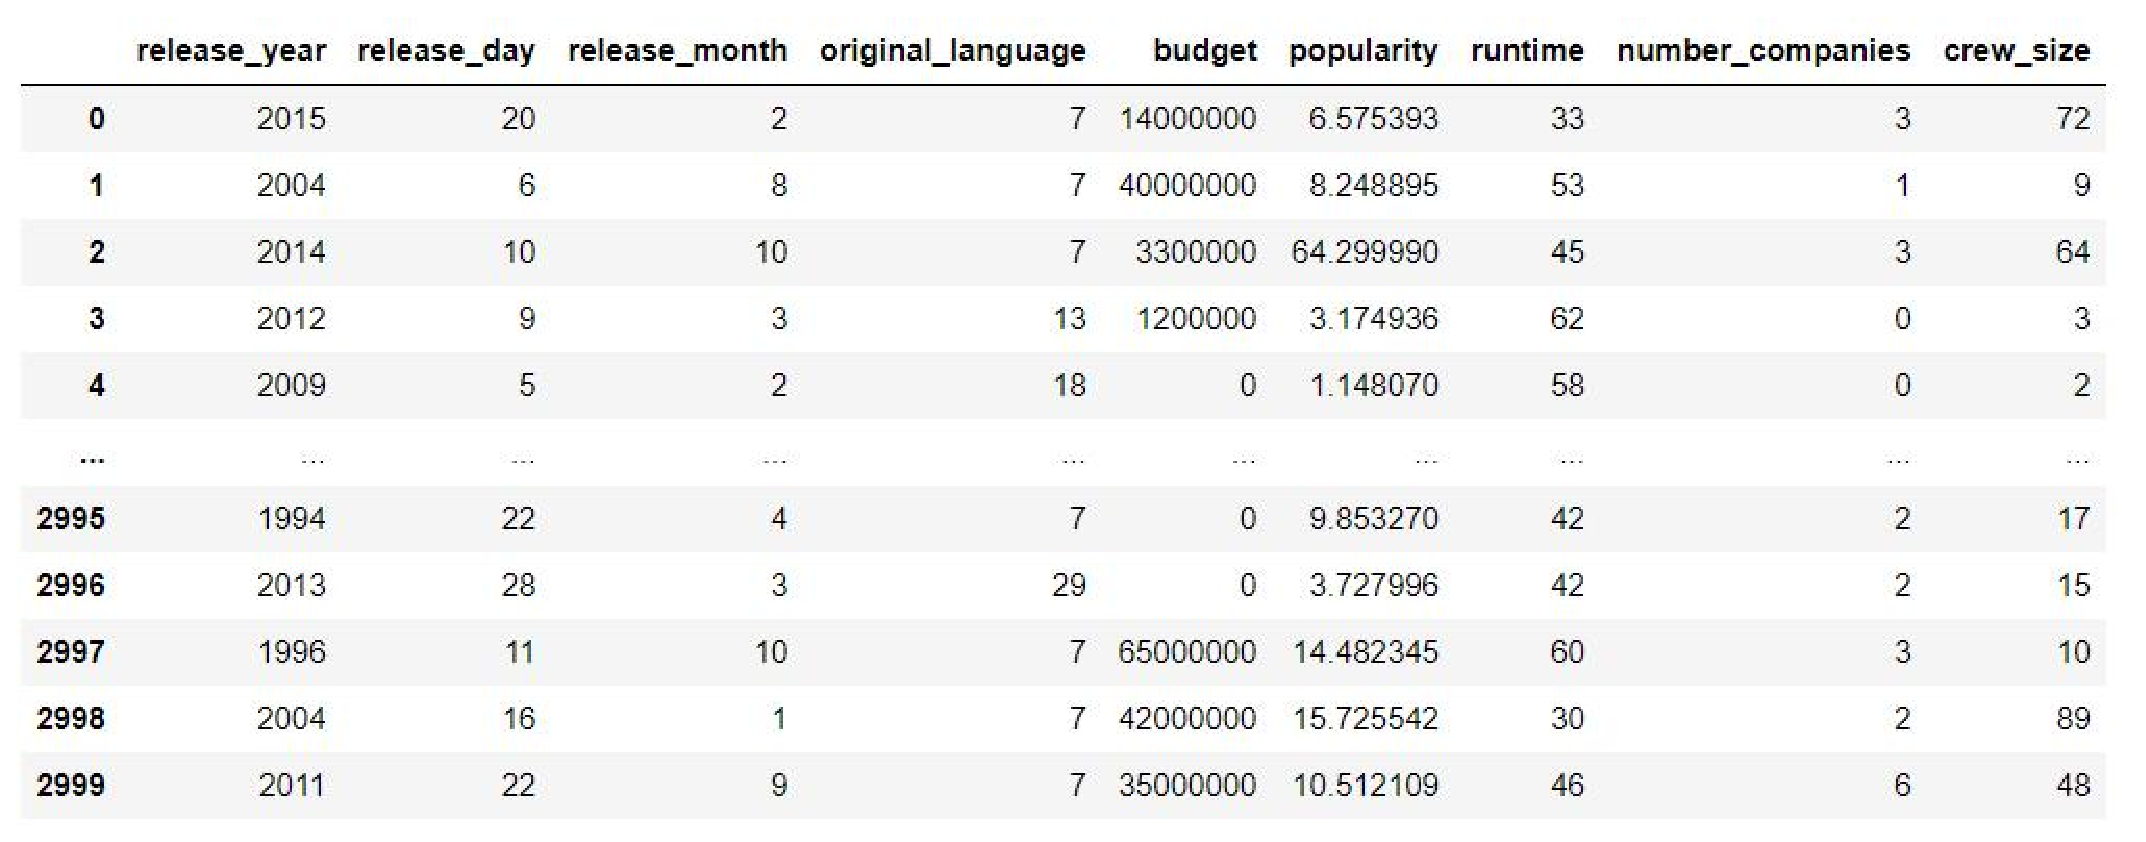
\includegraphics[width=0.6\textwidth,height=0.42\textwidth]{figures/feature1.eps}\\
    \caption{Feature}
  \end{figure}
 %%==========================================================================================
\begin{note}
However,
there is such a phenomenon in real life.
Doctors desire to identify the characteristics between
a group of cancer patients and normal people.
NBA coaches are passionate about exploring the obvious strengths and
weaknesses of the team compared with other teams.

Based on such a phenomenon in the real life,
we proposed the concept of group outlying aspects mining.
\end{note}
%%==========================================================================================
\end{slide}

%%==========================================================================================
%%
\begin{slide}{Model And Result}
  \begin{itemize}
    \item
    Random Forest
    \begin{itemize}
      \item
      A random forest is a classifier that contains multiple decision trees and whose
output class is determined by the plurality of the classes of the individual tree
outputs.
    \end{itemize}
    \item
    RMSE
    \begin{itemize}
      \item
      The root mean square error is the square root of the ratio of the deviation
       between the predicted value and the true value to the number of observations n.
    \end{itemize}
    \item
    Train set: 0.8 , Test set: 0.2
    \item
    Score:1.19
  \end{itemize}
 %%==========================================================================================
\begin{note}
However,
there is such a phenomenon in real life.
Doctors desire to identify the characteristics between
a group of cancer patients and normal people.
NBA coaches are passionate about exploring the obvious strengths and
weaknesses of the team compared with other teams.

Based on such a phenomenon in the real life,
we proposed the concept of group outlying aspects mining.
\end{note}
%%==========================================================================================
\end{slide}

\end{document}

\endinput
